\chapter{Волновые движения в замкнутом резервуаре при воздействии с двумя частотами}



Известно, что в океане существует великое множество волн. Вопрос будут ли волны различных частот мешать образовываться аттрактору до сих пор остается открытым. В данной работе изучается вопрос совместного воздействия на стратифицированную жидкость волнопродуктора с двумя различными частотами и одинаковой амплитудой. 

Постановка задачи несколько меняется. Для моделирования используется конфигурация представленная на рисунке \ref{fig:domainup}. Условие на волнопродукторе будет теперь записываться следующим образом:

\begin{equation}
    U_z = A_1\cdot cos\left(\frac{\pi \cdot z}{L_1}\right)\cdot \omega_1 \cdot  sin(\omega_1 t) + A_2\cdot cos\left(\frac{\pi \cdot z}{L_1}\right)\cdot \omega_2 \cdot  sin(\omega_2 t)
\end{equation}

Посчитаны различные режимы:

\begin{itemize}
    \item Режим разнесенными частотами, $\omega_1/N=0.58$ $\omega_2/N=0.66$ и малой амплитудой $a=0.02$ см. 
    \item Режим с совпадающими частотами, $\omega_1=\omega_2=0.628$ и амплитудой $a=0.05$ см.
    \item Режим с приближенными частотами, $\omega_1/N=0.66$ $\omega_2/N=0.68$ и амплитудой $a=0.05$ см.
    \item Режим с близкими частотами $\omega_1/N=0.628$ $\omega_2/N=0.641$ и  амплитудой $a=0.05$ см.
\end{itemize}

Первый режим демонстрирует общую картину течения при взаимодействии с двумя частотами. На рисунке \ref{fig:biharmVyamp02} показано, что в одном резервуаре допустимо существования сразу двух аттракторов внутренних волн. Это видно по характерному распределению поля скоростей и давлений в резервуаре. В середине первого(том что соединяет нижнюю и наклонную стенку) луче аттрактора помещена точка пробы. Видно, что существует задержка между частотой колебания волнопродуктора и частотой колебаний в середине первого луча аттрактора. Помимо этого, построен спектр частот колебаний скорости, частоты на этом графике осреднены по большей из частот. Сама точка пробы также размещена на первом луче аттрактора, который возникает под воздействием большей из частот. Это объясняет то почему второй пик меньше. На протяжении всей частотно-временной диаграммы наблюдается доминация этих двух частот.

\begin{figure}
  \centering
    \begin{subfigure}[с]{0.45\textwidth}
        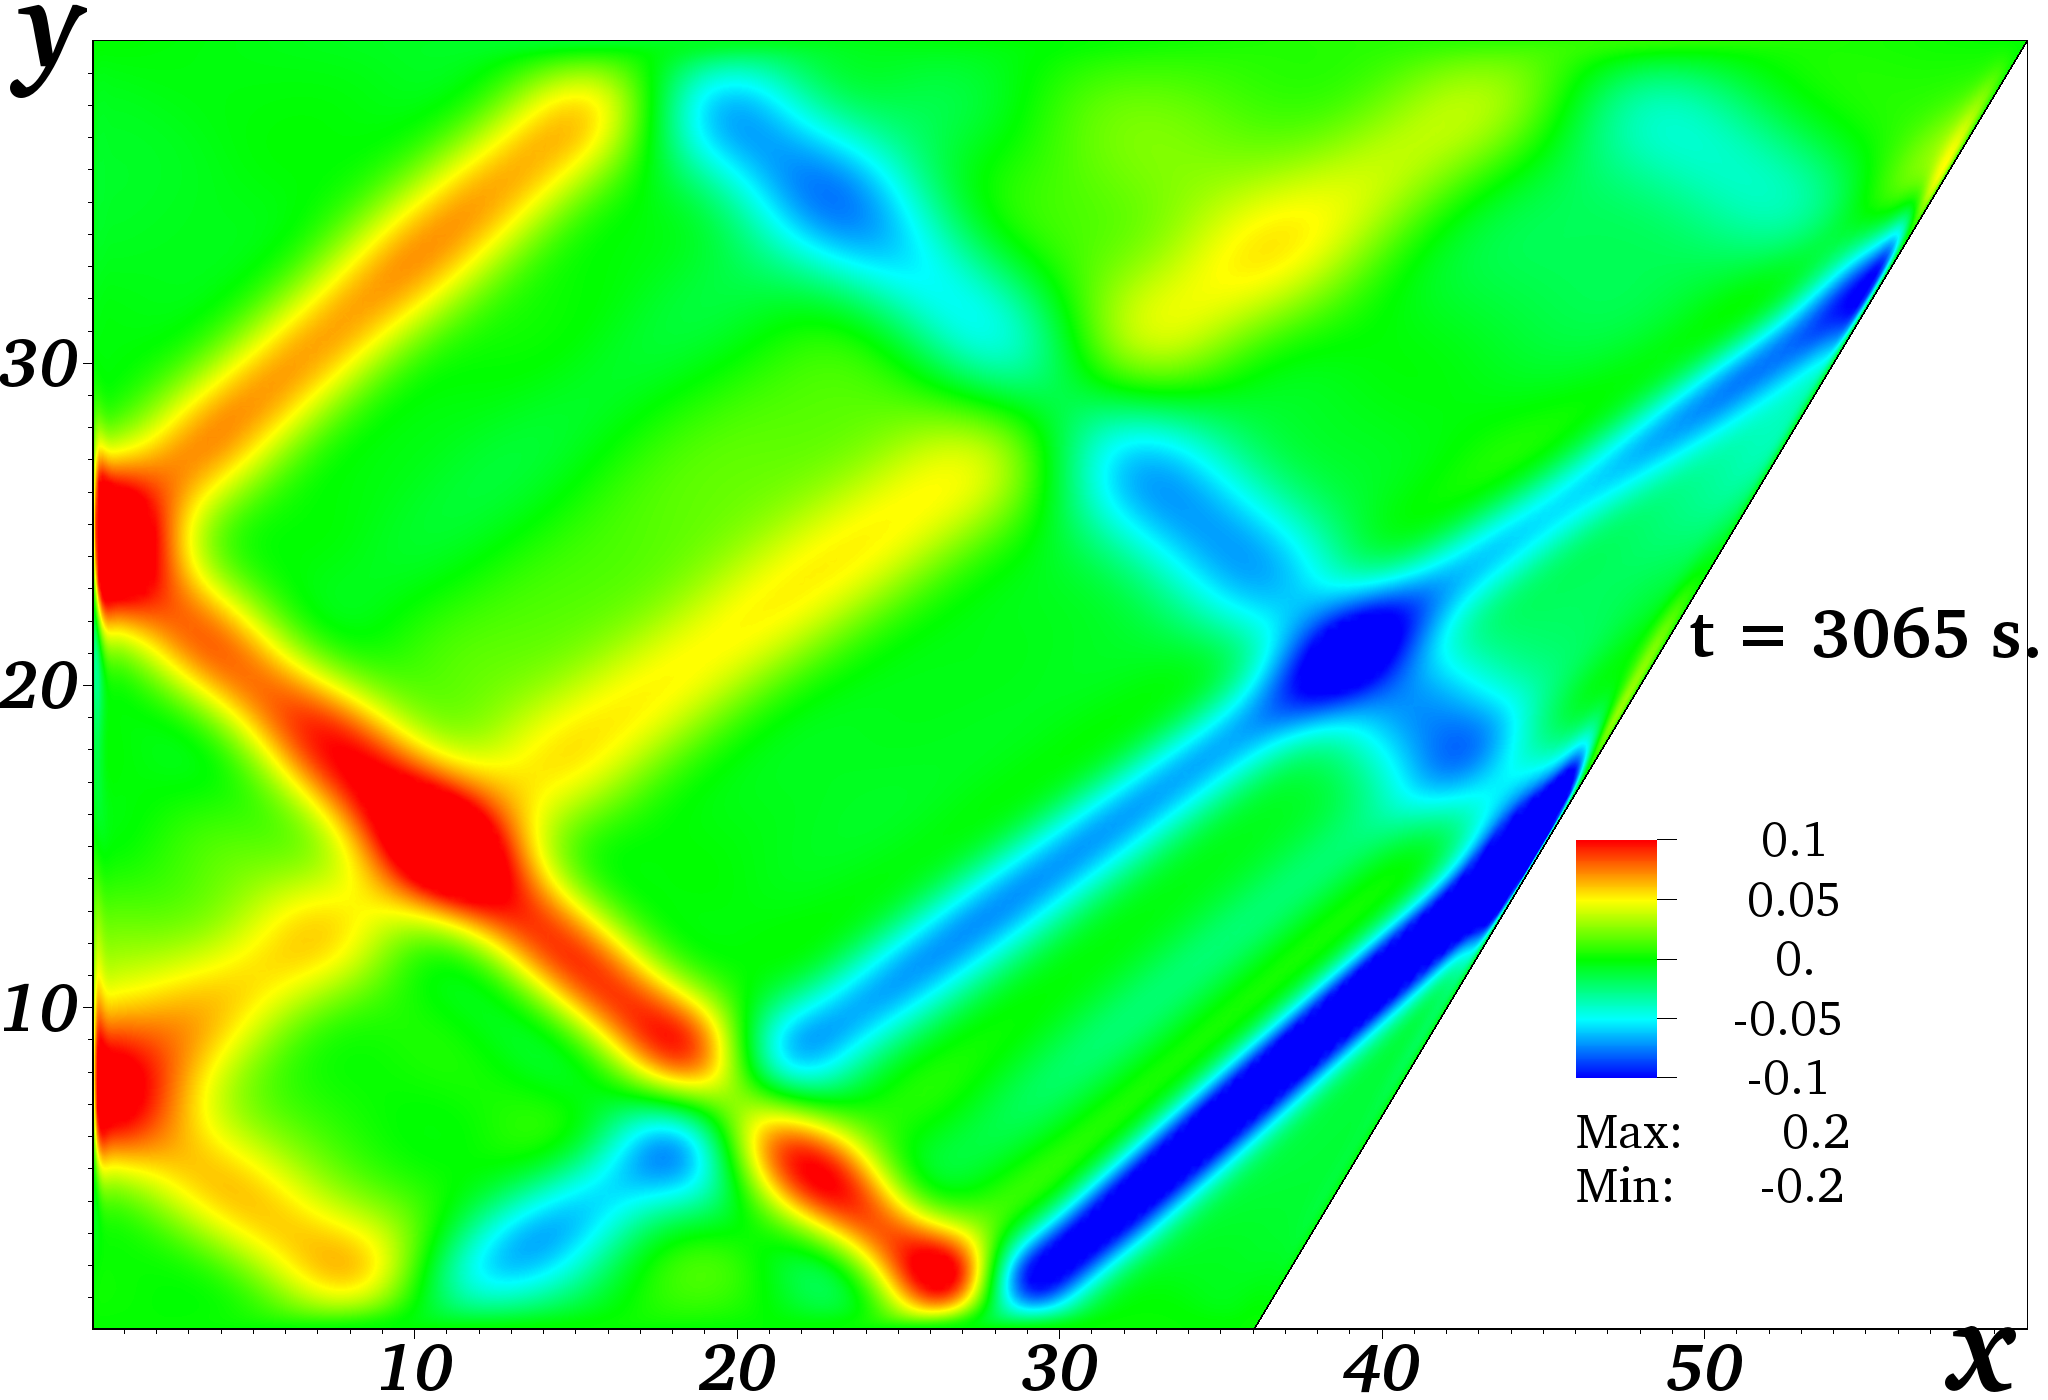
\includegraphics[width=1\textwidth]{pics/H40L60N1ap02dp20w1p58w2p66Biharm/2D36x36DiagramH40L60N1ap02dp20w1p58w2p66BiharmVyn06129.png}
        \caption{Вертикальная компонента скорости}
    \end{subfigure}
    \begin{subfigure}[с]{0.45\textwidth}
        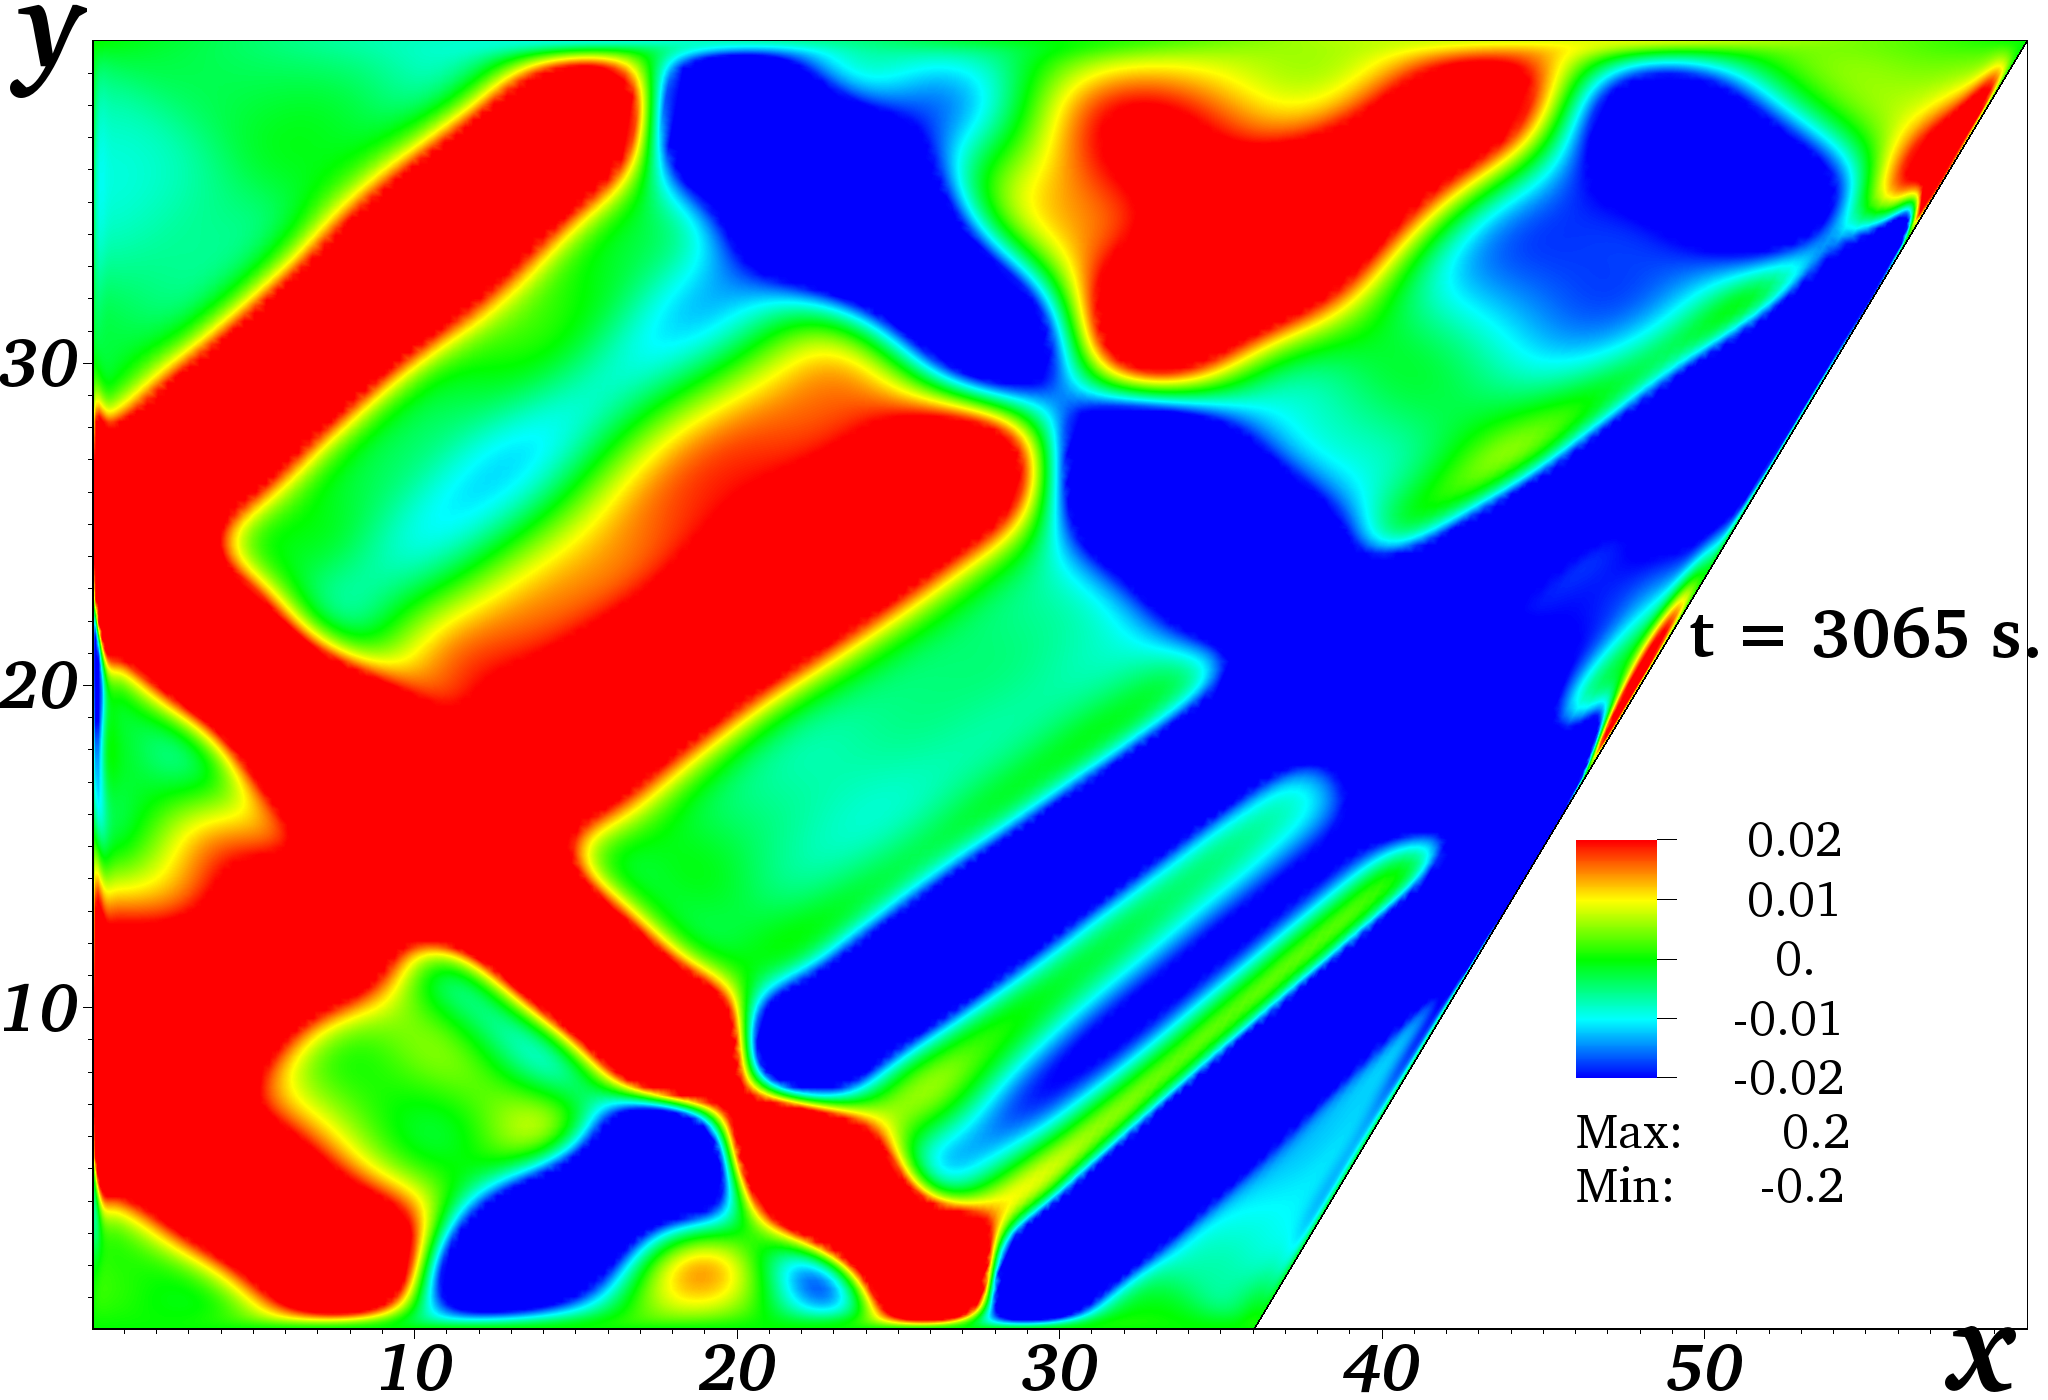
\includegraphics[width=1\textwidth]{pics/H40L60N1ap02dp20w1p58w2p66Biharm/2D36x36DiagramH40L60N1ap02dp20w1p58w2p66BiharmVy6129.png}
        \caption{Поле давления}
    \end{subfigure}
    \par
    \begin{subfigure}[с]{0.45\textwidth}
        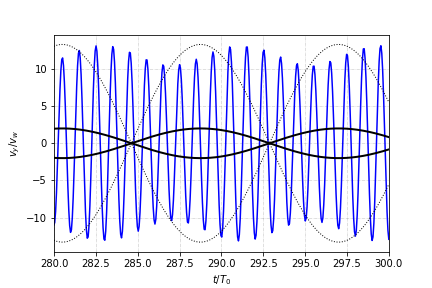
\includegraphics[width=1\textwidth]{pics/H40L60N1ap02dp20w1p58w2p66Biharm/vyX36p49Y7p94frm280to300.png}
        \caption{Вертикальная компонента скорости в середине первого луча аттрактора}
    \end{subfigure}
    \begin{subfigure}[с]{0.45\textwidth}
        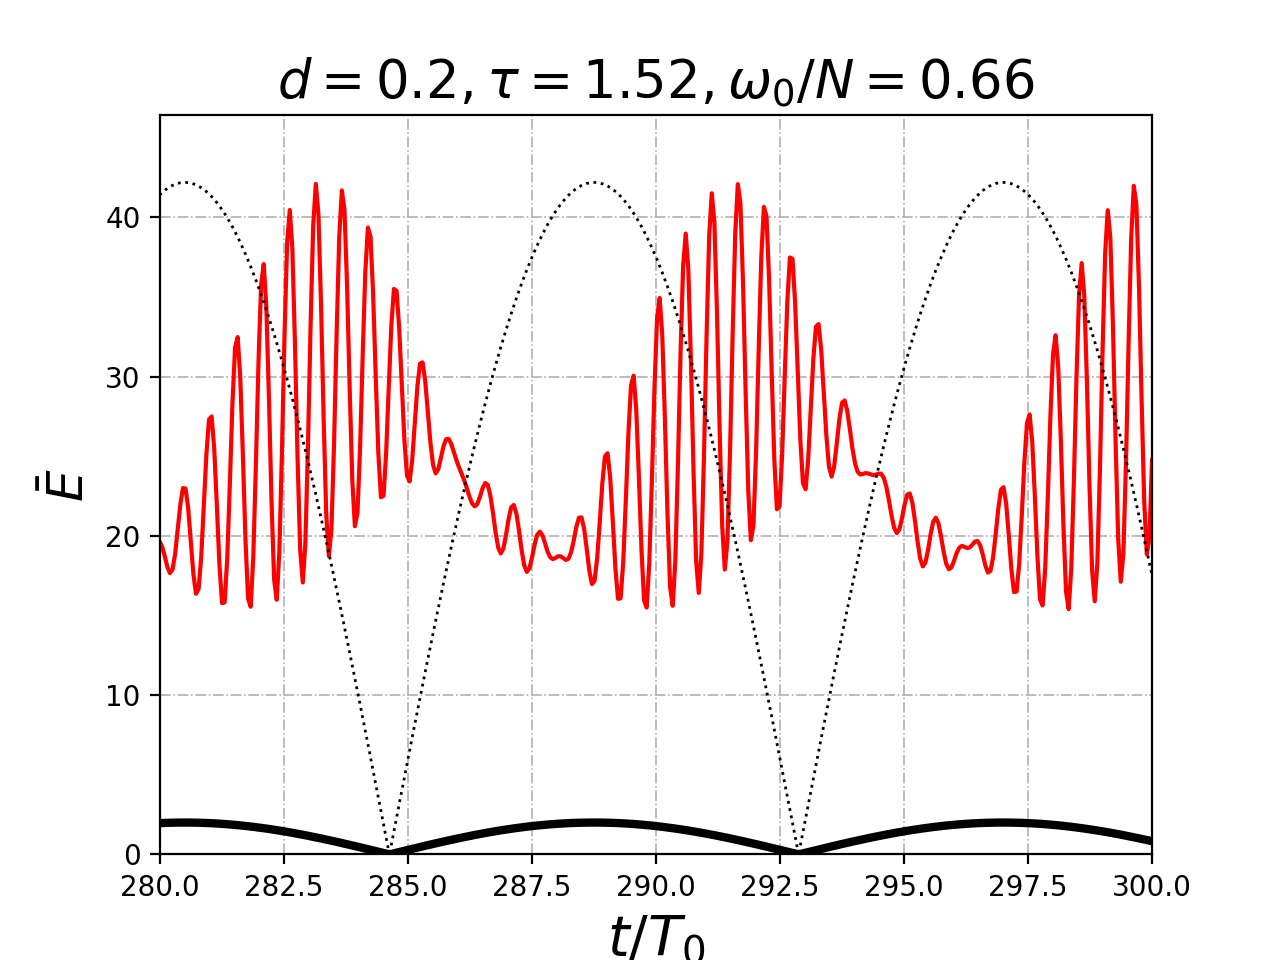
\includegraphics[width=1\textwidth]{pics/H40L60N1ap02dp20w1p58w2p66Biharm/2D36x36DiagramH40L60N1ap02dp20w1p58w2p66BiharmtotKEnonDim.png}
        \caption{Средняя кинетическая энергия в резервуаре}
    \end{subfigure}
    \par
    \begin{subfigure}[с]{0.45\textwidth}
        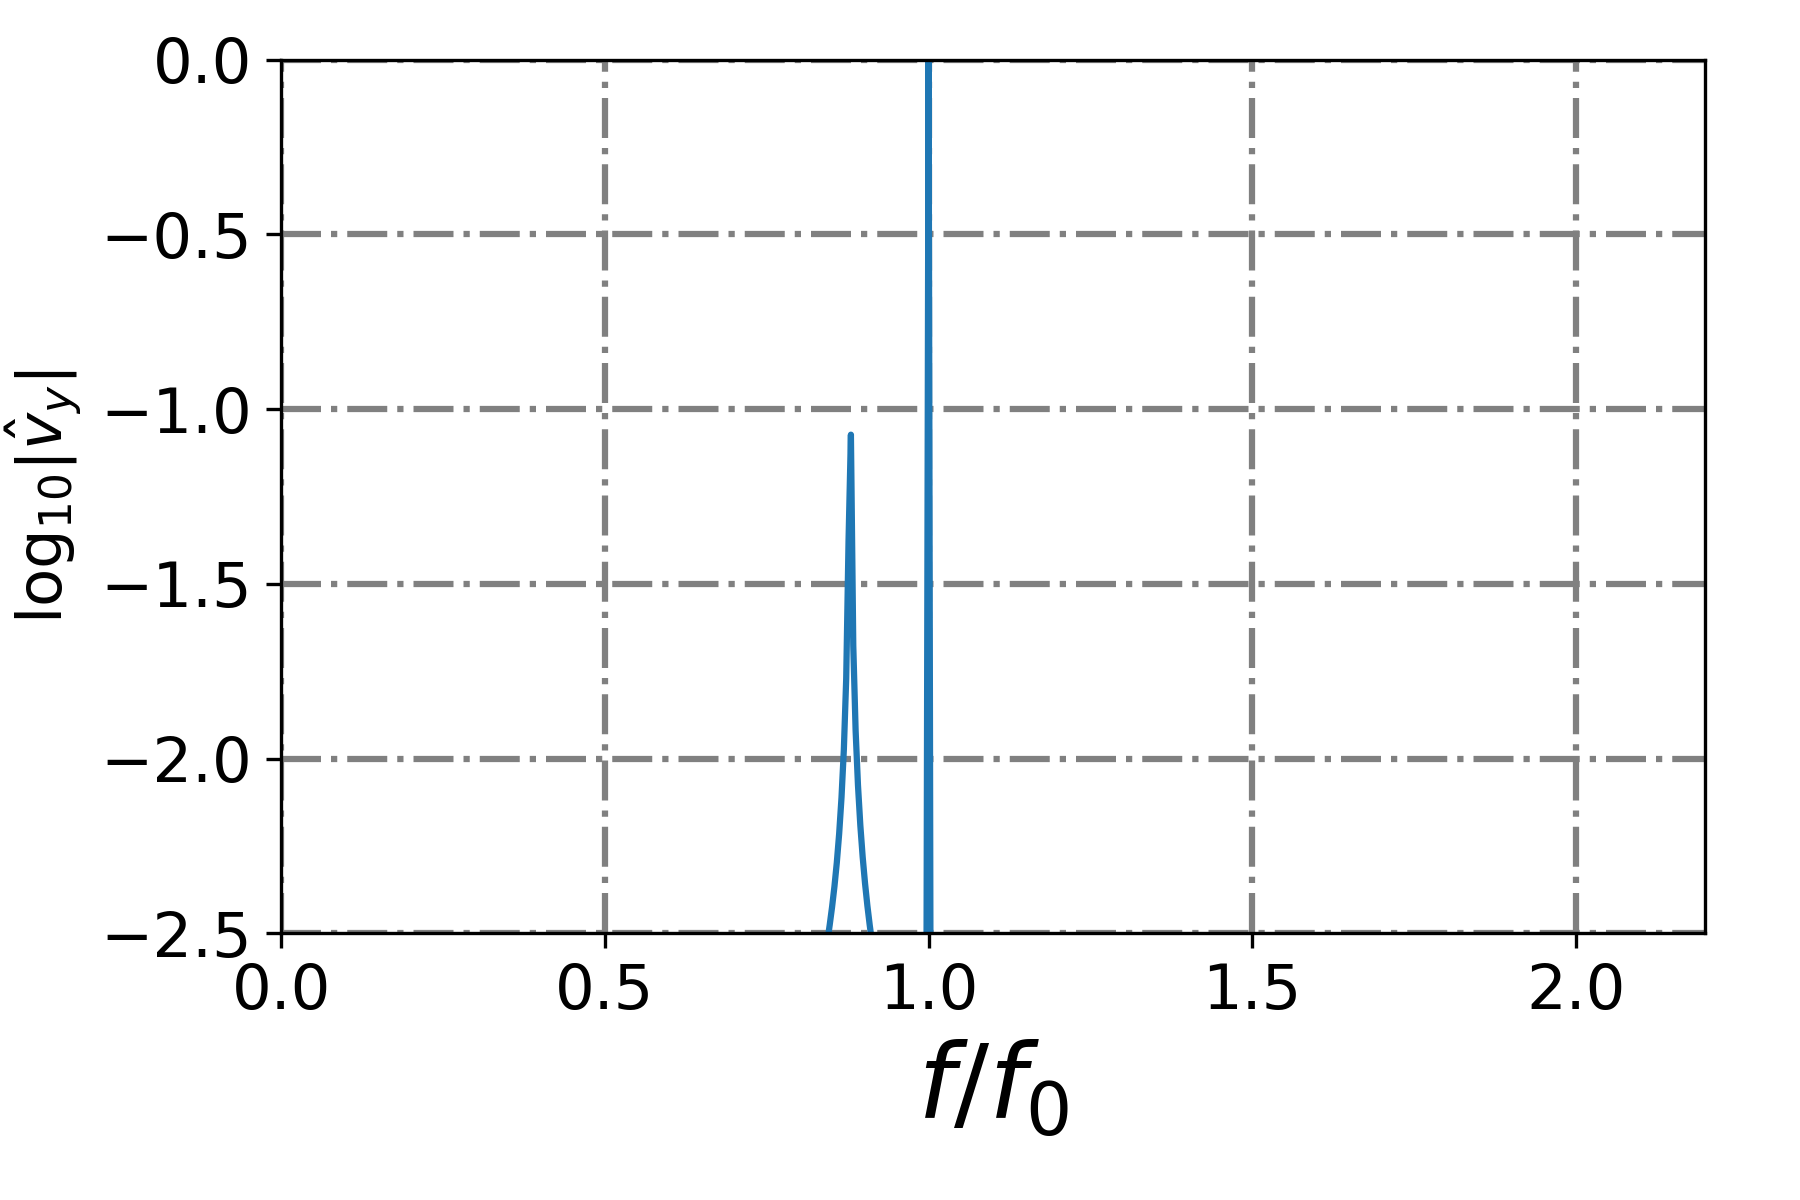
\includegraphics[width=1\textwidth]{pics/H40L60N1ap02dp20w1p58w2p66Biharm/spectrumX36p4Y8p0.png}
        \caption{Спектр}
    \end{subfigure}
    \begin{subfigure}[с]{0.45\textwidth}
        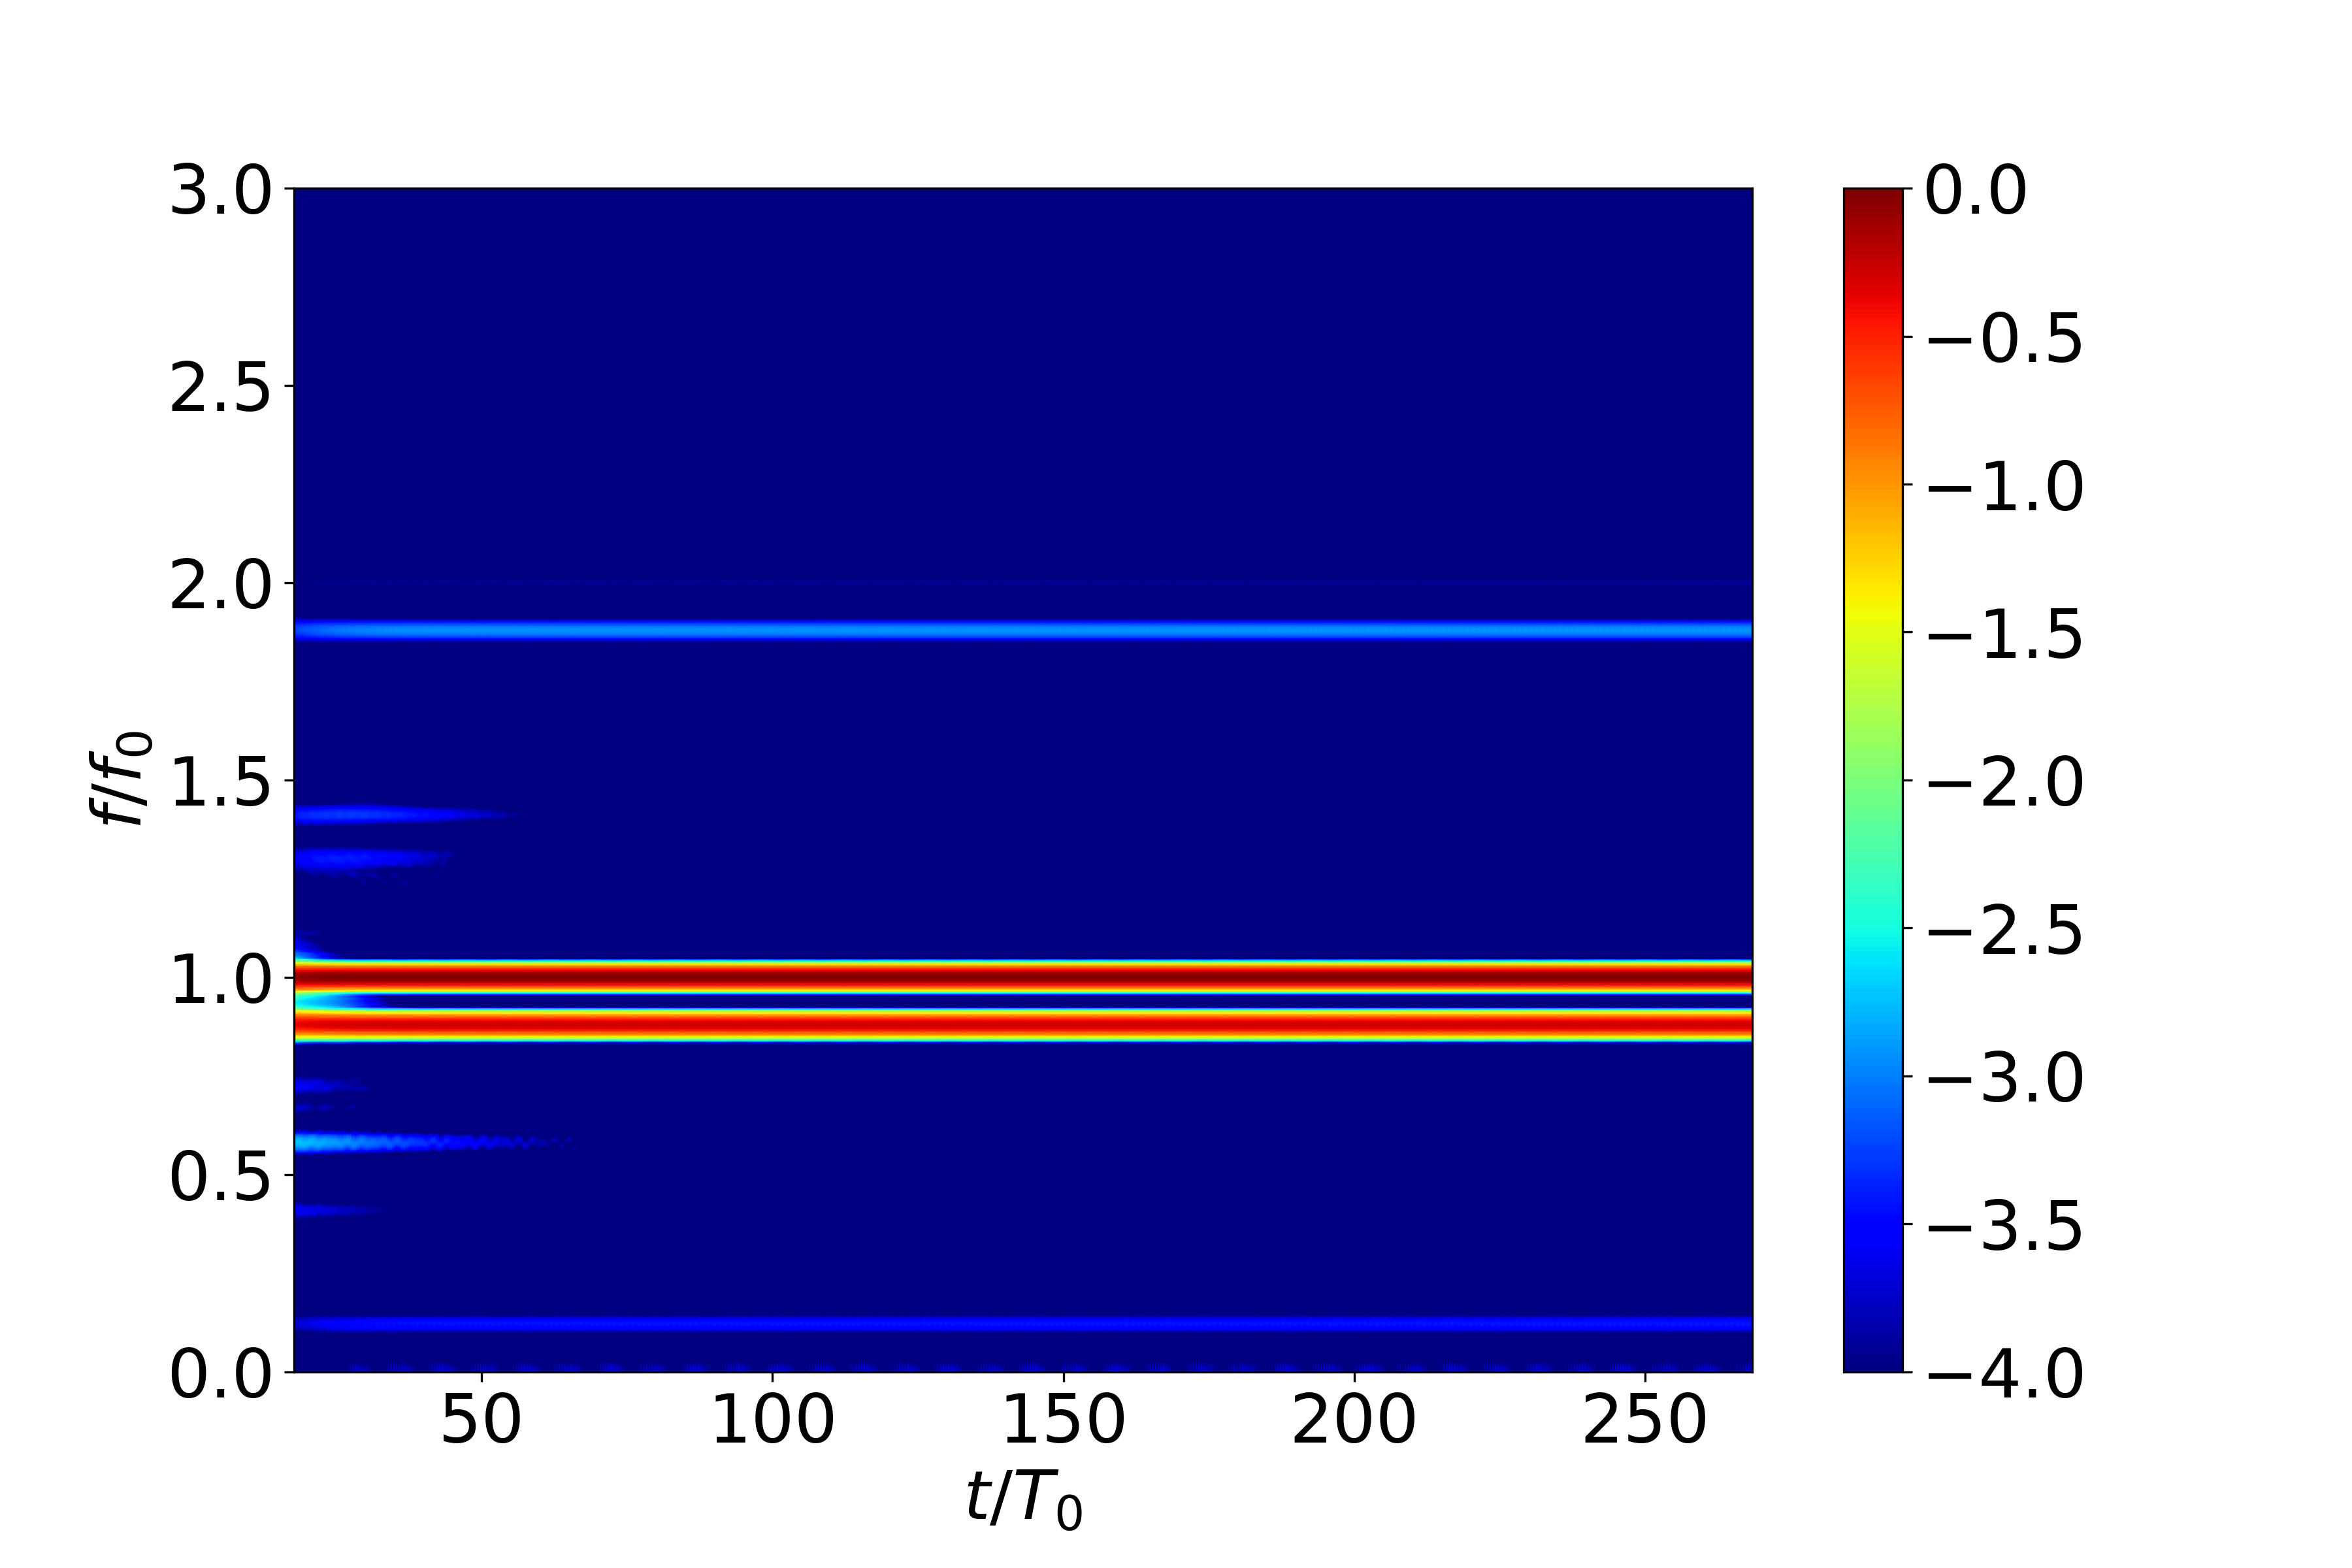
\includegraphics[width=1\textwidth]{pics/H40L60N1ap02dp20w1p58w2p66Biharm/TFspectrumX36p4Y8p0N768.png}
        \caption{Частотно-временная диаграмма}
    \end{subfigure}
    \caption{Результаты количественного исследования характеристик течения стратифицированной жидкости в трапециевидном резервуаре при внешнем воздействии с двумя разнесенными частотами $\omega_1/N=0.58$,  $\omega_2/N=0.66$. Черной линией  на графиках вертикальной скорости и кинетической энергии показана огибающая амплитуды колебаний волнпородуктора.}
    \label{fig:biharmVyamp02}
\end{figure}

Совпадение частот означает, что амплитуда колебаний удваивается значение $a=0.05$ cm. При $a=0.1$ на рисунке \ref{fig:Vyamp1} наблюдается неустойчивость этот режим характеризуется россыпью частот на спектре и частотно-временной диаграмме.

\begin{figure}
	\centering
	\begin{subfigure}[с]{0.45\textwidth}
	    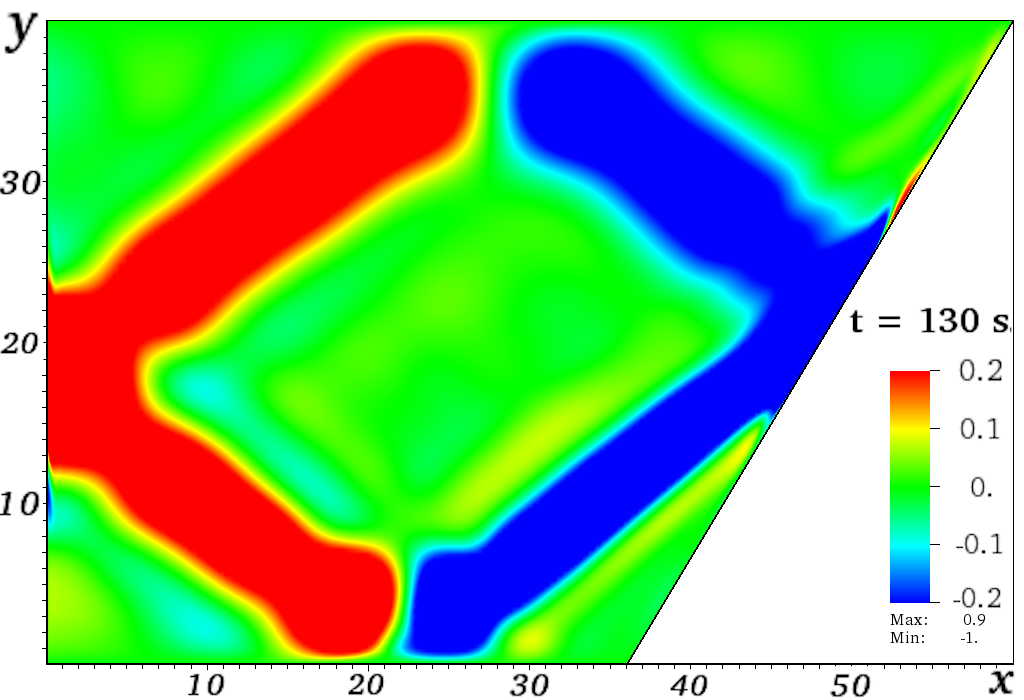
\includegraphics[width=1\textwidth]{pics/H40L60N1ap10dp20w0p63/2DH40L60N1ap10dp20w0p63Vyn00012.png}
	    \caption{Поле вертикальной скорости при образовании аттрактора}
	\end{subfigure}
	\begin{subfigure}[с]{0.45\textwidth}
	    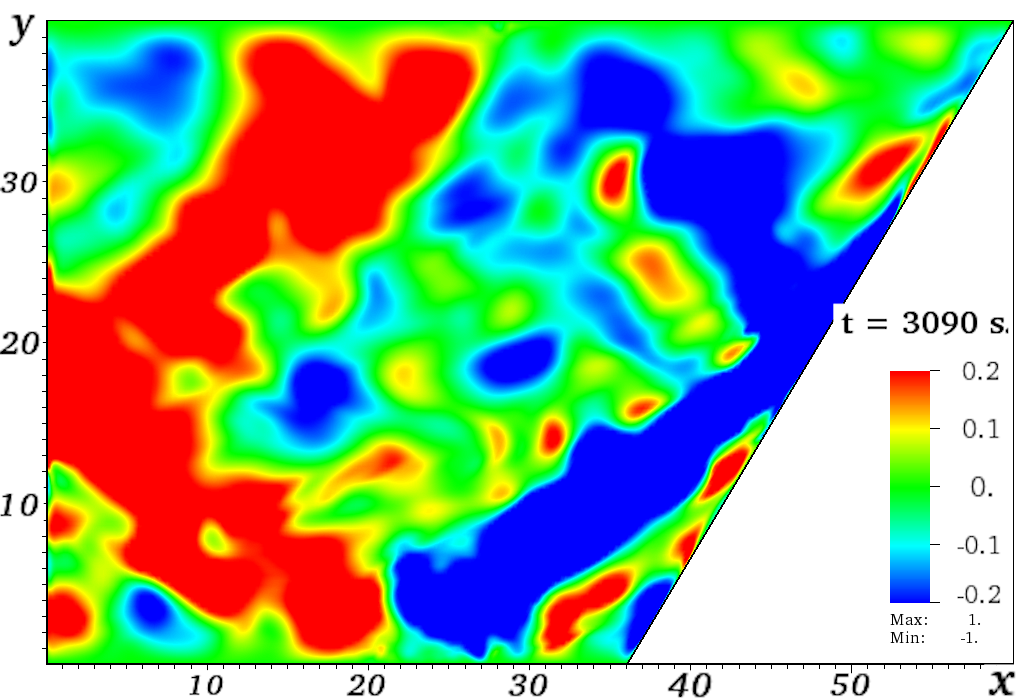
\includegraphics[width=1\textwidth]{pics/H40L60N1ap10dp20w0p63/2DH40L60N1ap10dp20w0p63Vyn00308.png}
	    \caption{Поле вертикальной скорости при образовании неустойчивостей}
	\end{subfigure}
	\par
	\begin{subfigure}[с]{0.45\textwidth}
	    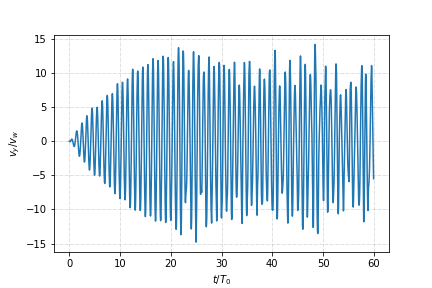
\includegraphics[width=1\textwidth]{pics/H40L60N1ap10dp20w0p63/vyX35p6Y11p3t1200.png}
	    \caption{зависимость скорости в середине первого луча аттрактора от времени}
	\end{subfigure}
	\begin{subfigure}[с]{0.45\textwidth}
	    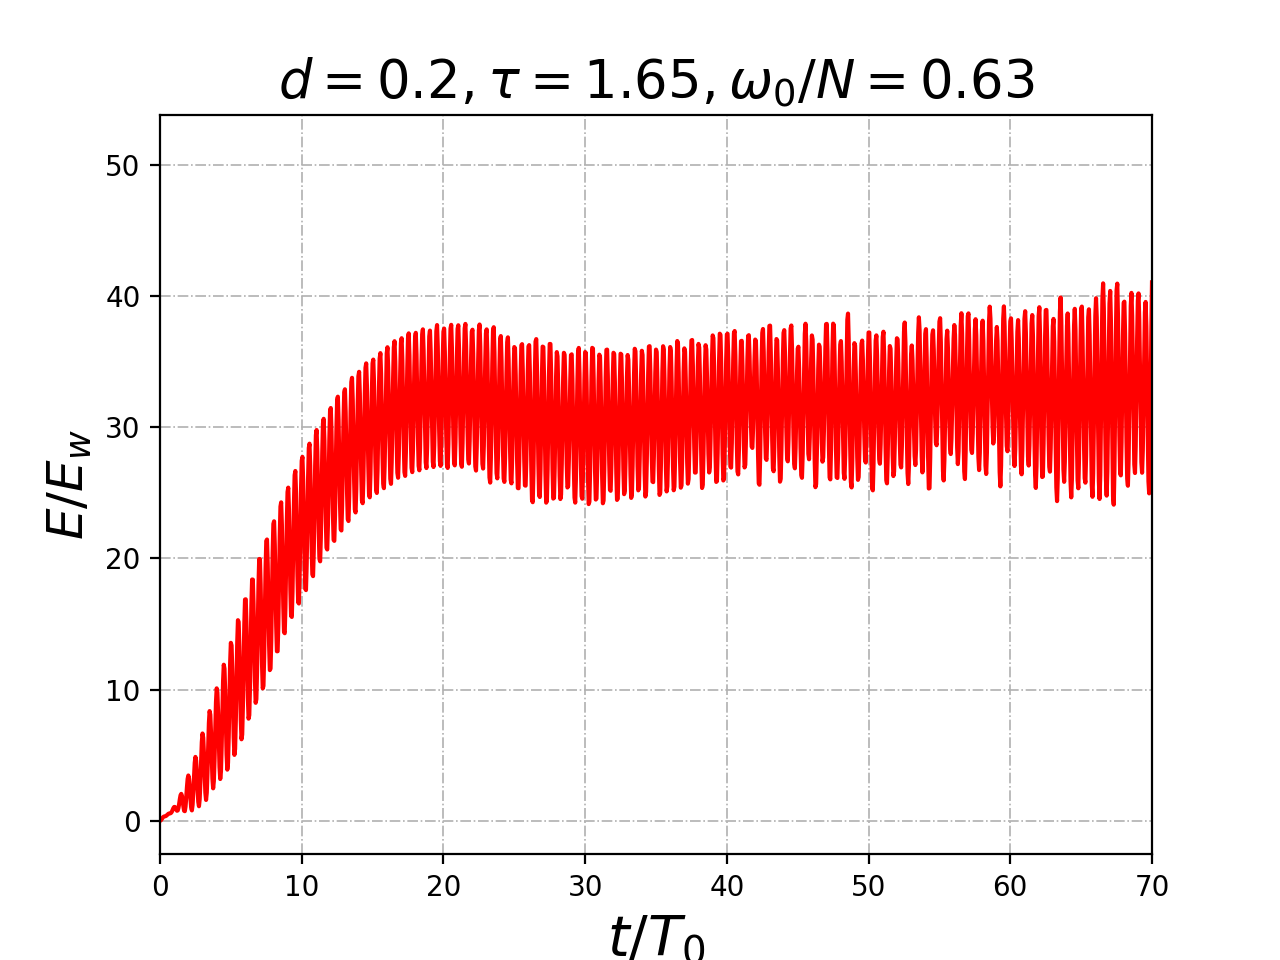
\includegraphics[width=1\textwidth]{pics/H40L60N1ap10dp20w0p63/2D36x36DiagramH40L60N1ap10dp20w0p63totKEnonDim.png}
	    \caption{Зависимость кинетической энергии от времени}
	\end{subfigure}
	\par
	\begin{subfigure}[с]{0.45\textwidth}
	    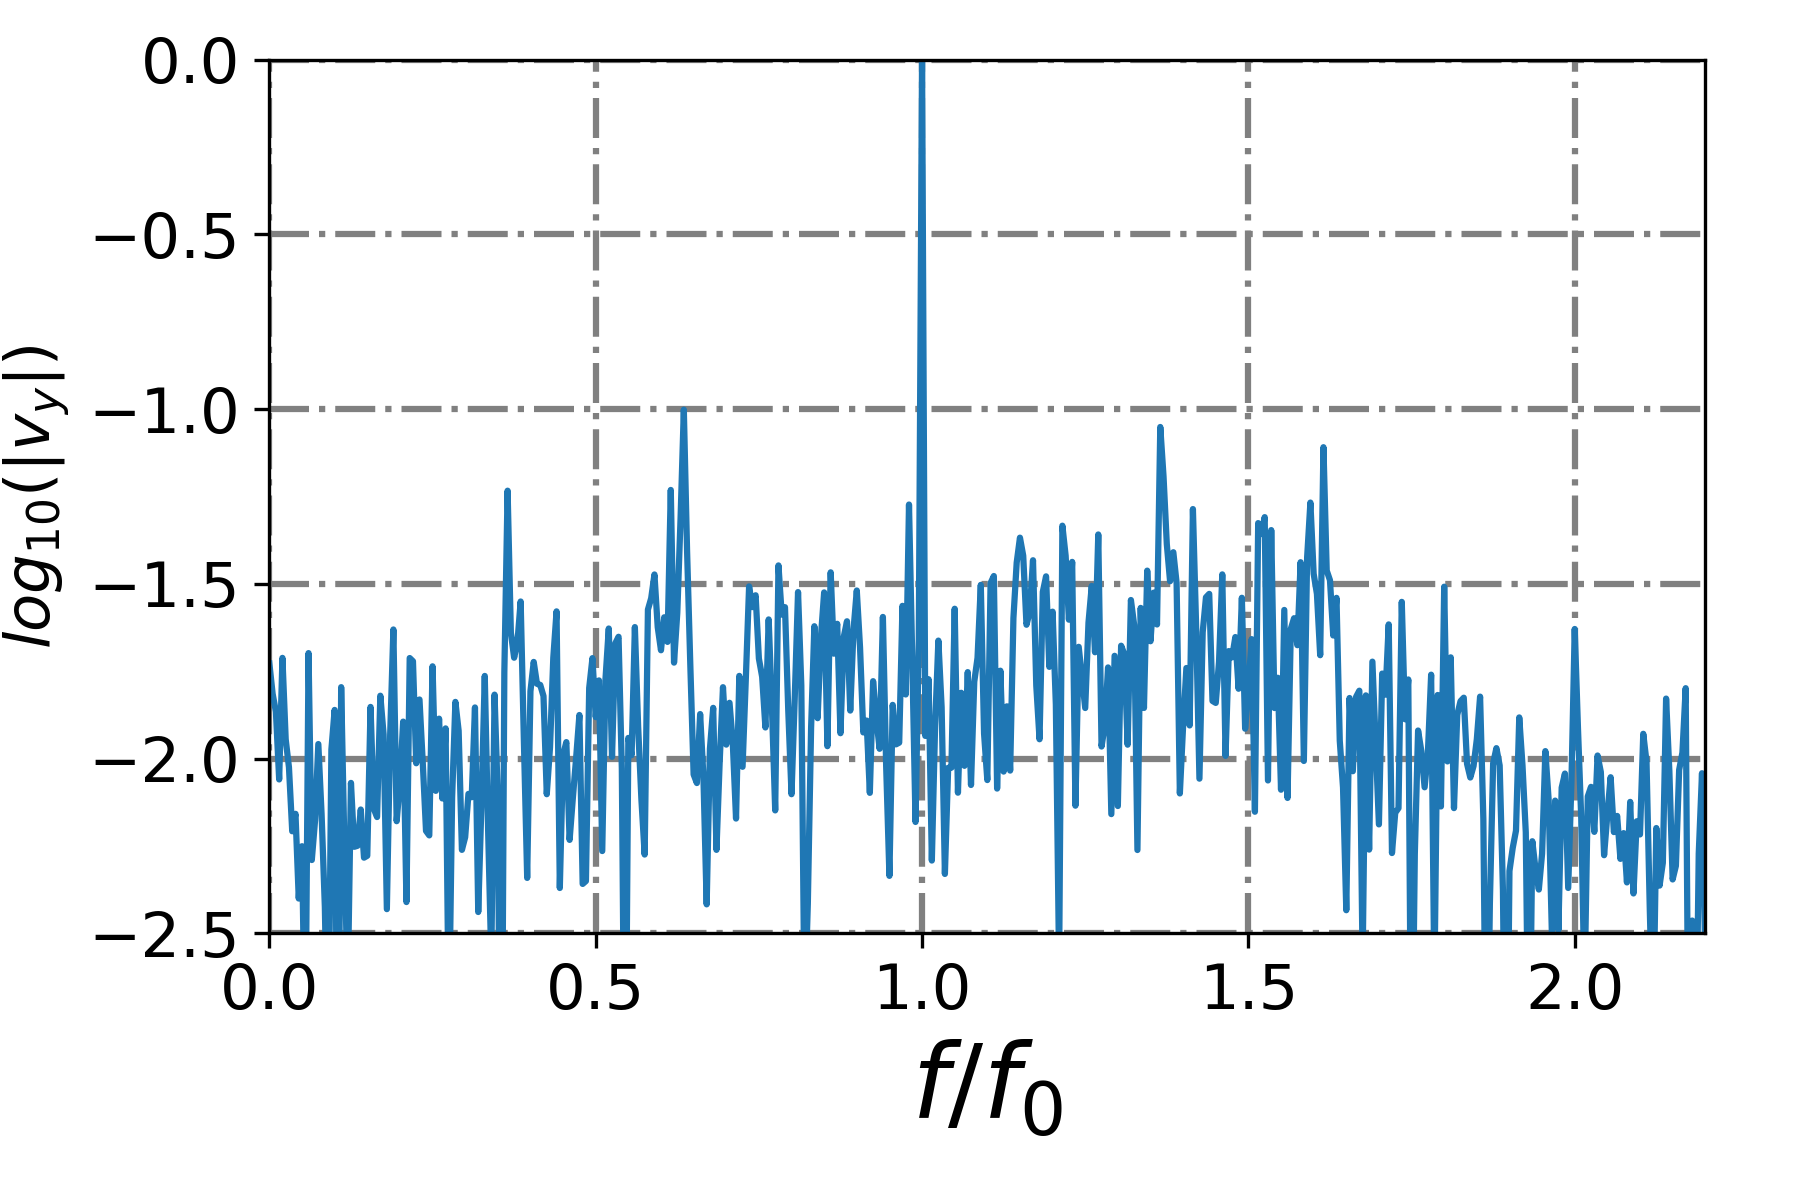
\includegraphics[width=1\textwidth]{pics/H40L60N1ap10dp20w0p63/spectrumX35p6Y11p2n4000.png}
	    \caption{Частотный спектр скорости}
	\end{subfigure}
	\begin{subfigure}[с]{0.45\textwidth}
	    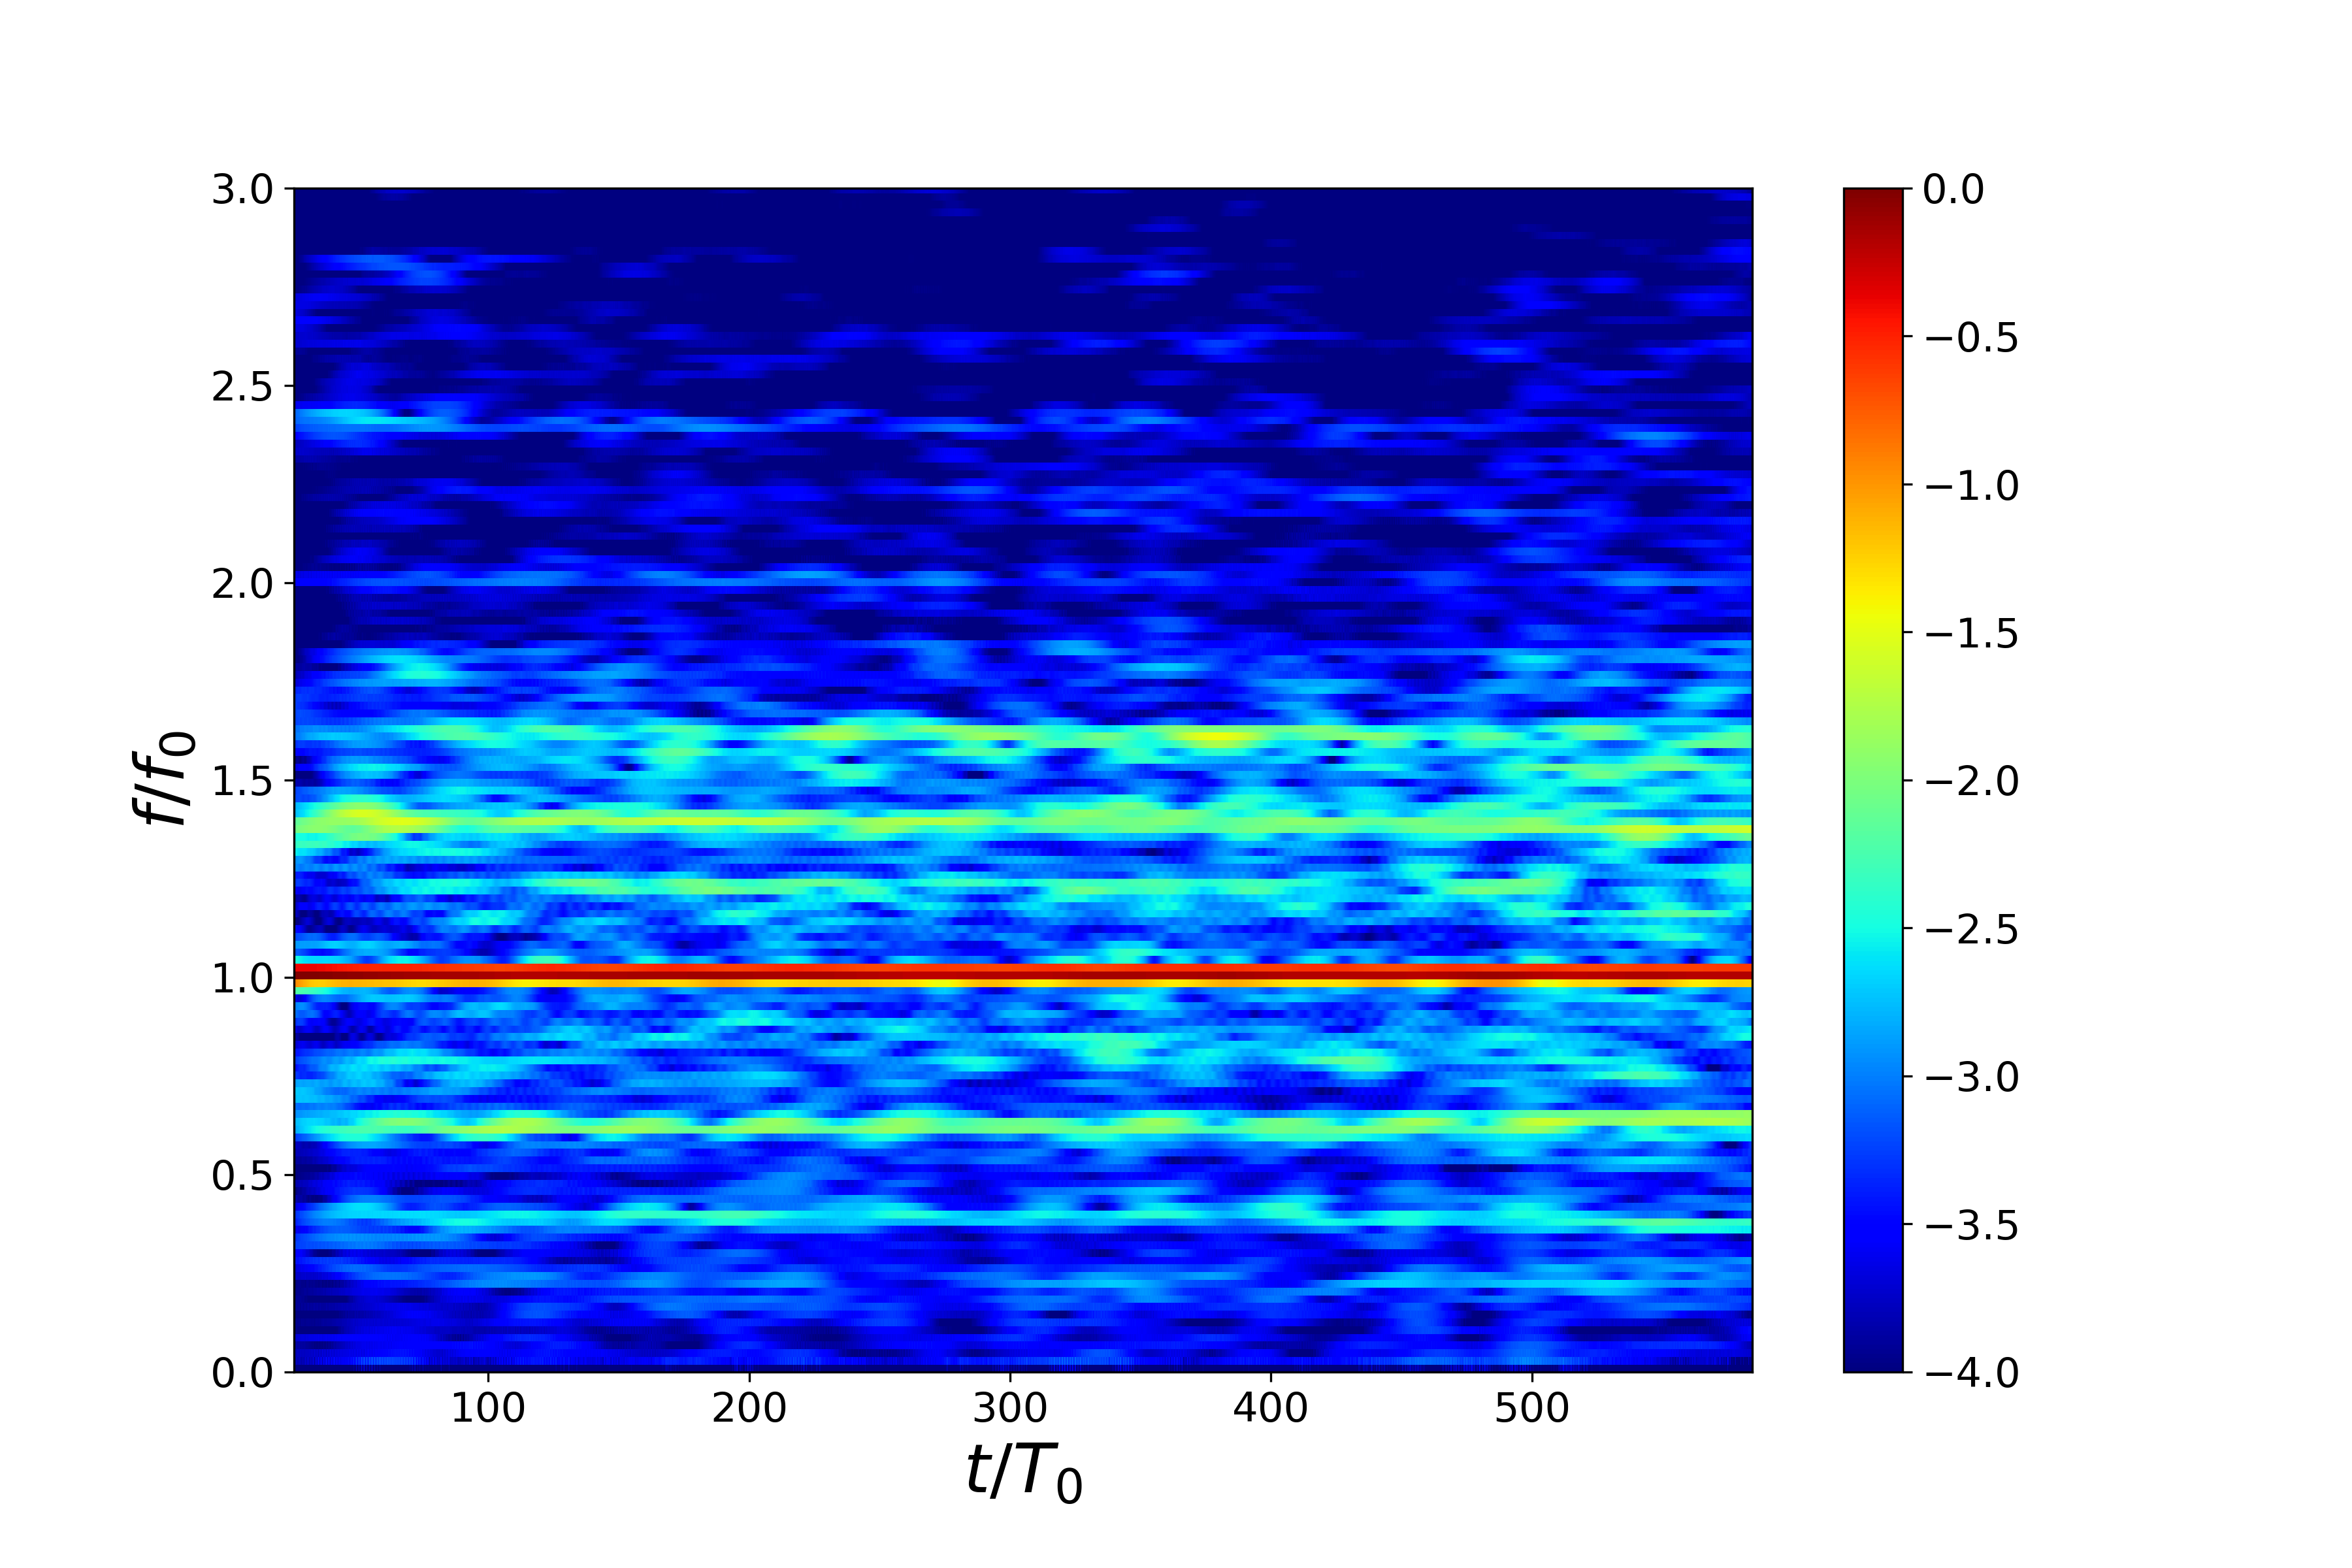
\includegraphics[width=1\textwidth]{pics/H40L60N1ap10dp20w0p63/TFspectrumX35p6Y11p2N1024.png}
	    \caption{Частотно-временная диаграмма}
	\end{subfigure}
	\label{fig:Vyamp1-1}
	\caption{Количественное исследования аттрактора с совпадающими частотами и образование неустойчивости}
	\label{fig:Vyamp1}
\end{figure}

Последующие режимы это попытка постепенно приблизить две частоты друг к другу и зафиксировать момент возникновения неустойчивости в зависимости от близости частот друг к другу. На рисунке \ref{fig:biharmVyap005-1} представлена картина течения при относительной разности частот в 0.05. При этом режиме наблюдаются дочерние волны как на изображении с вертикальной компонентой скорости, спектре так и на частотно временной диаграмме. При этом на последней наблюдаются  амплитудные <<всплески>>. Это объясняется совпадением фаз двух волновых процессов.

\begin{figure}
  \centering
  \begin{subfigure}[с]{0.45\textwidth}
    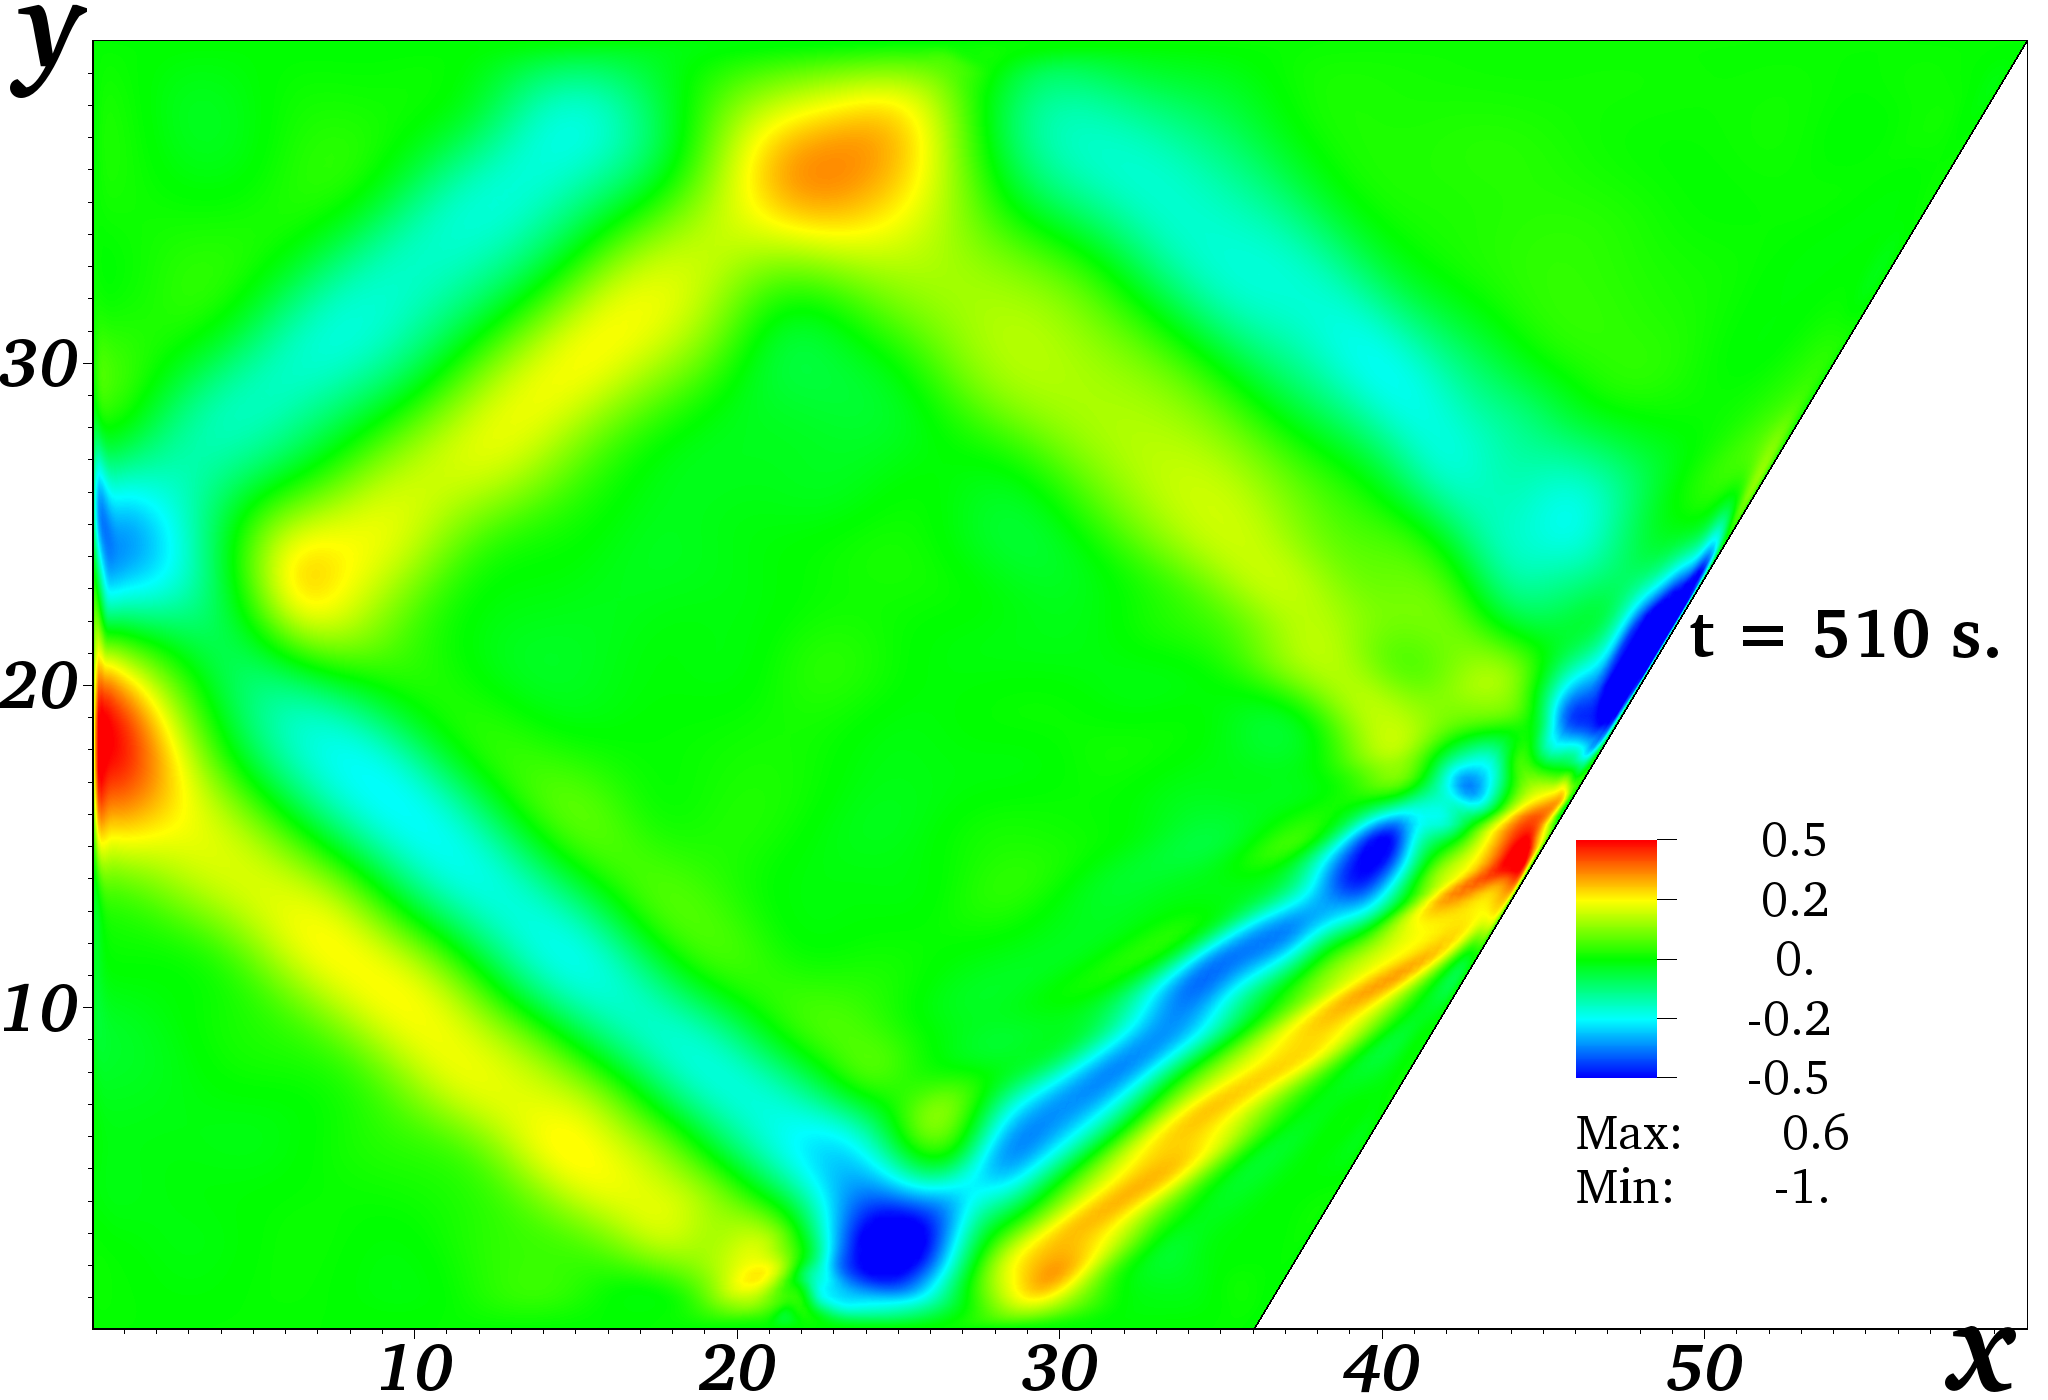
\includegraphics[width=1\textwidth]{pics/H40L60N1ap05dp20w1p63Deltawp05Biharm/2D36x36DiagramH40L60N1ap05dp20w0p63Deltawp3315BiharmVyn01019.png}
    \caption{Вертикальная компонента скорости при формировании аттрактора}
  \end{subfigure}
  \begin{subfigure}[с]{0.45\textwidth}
    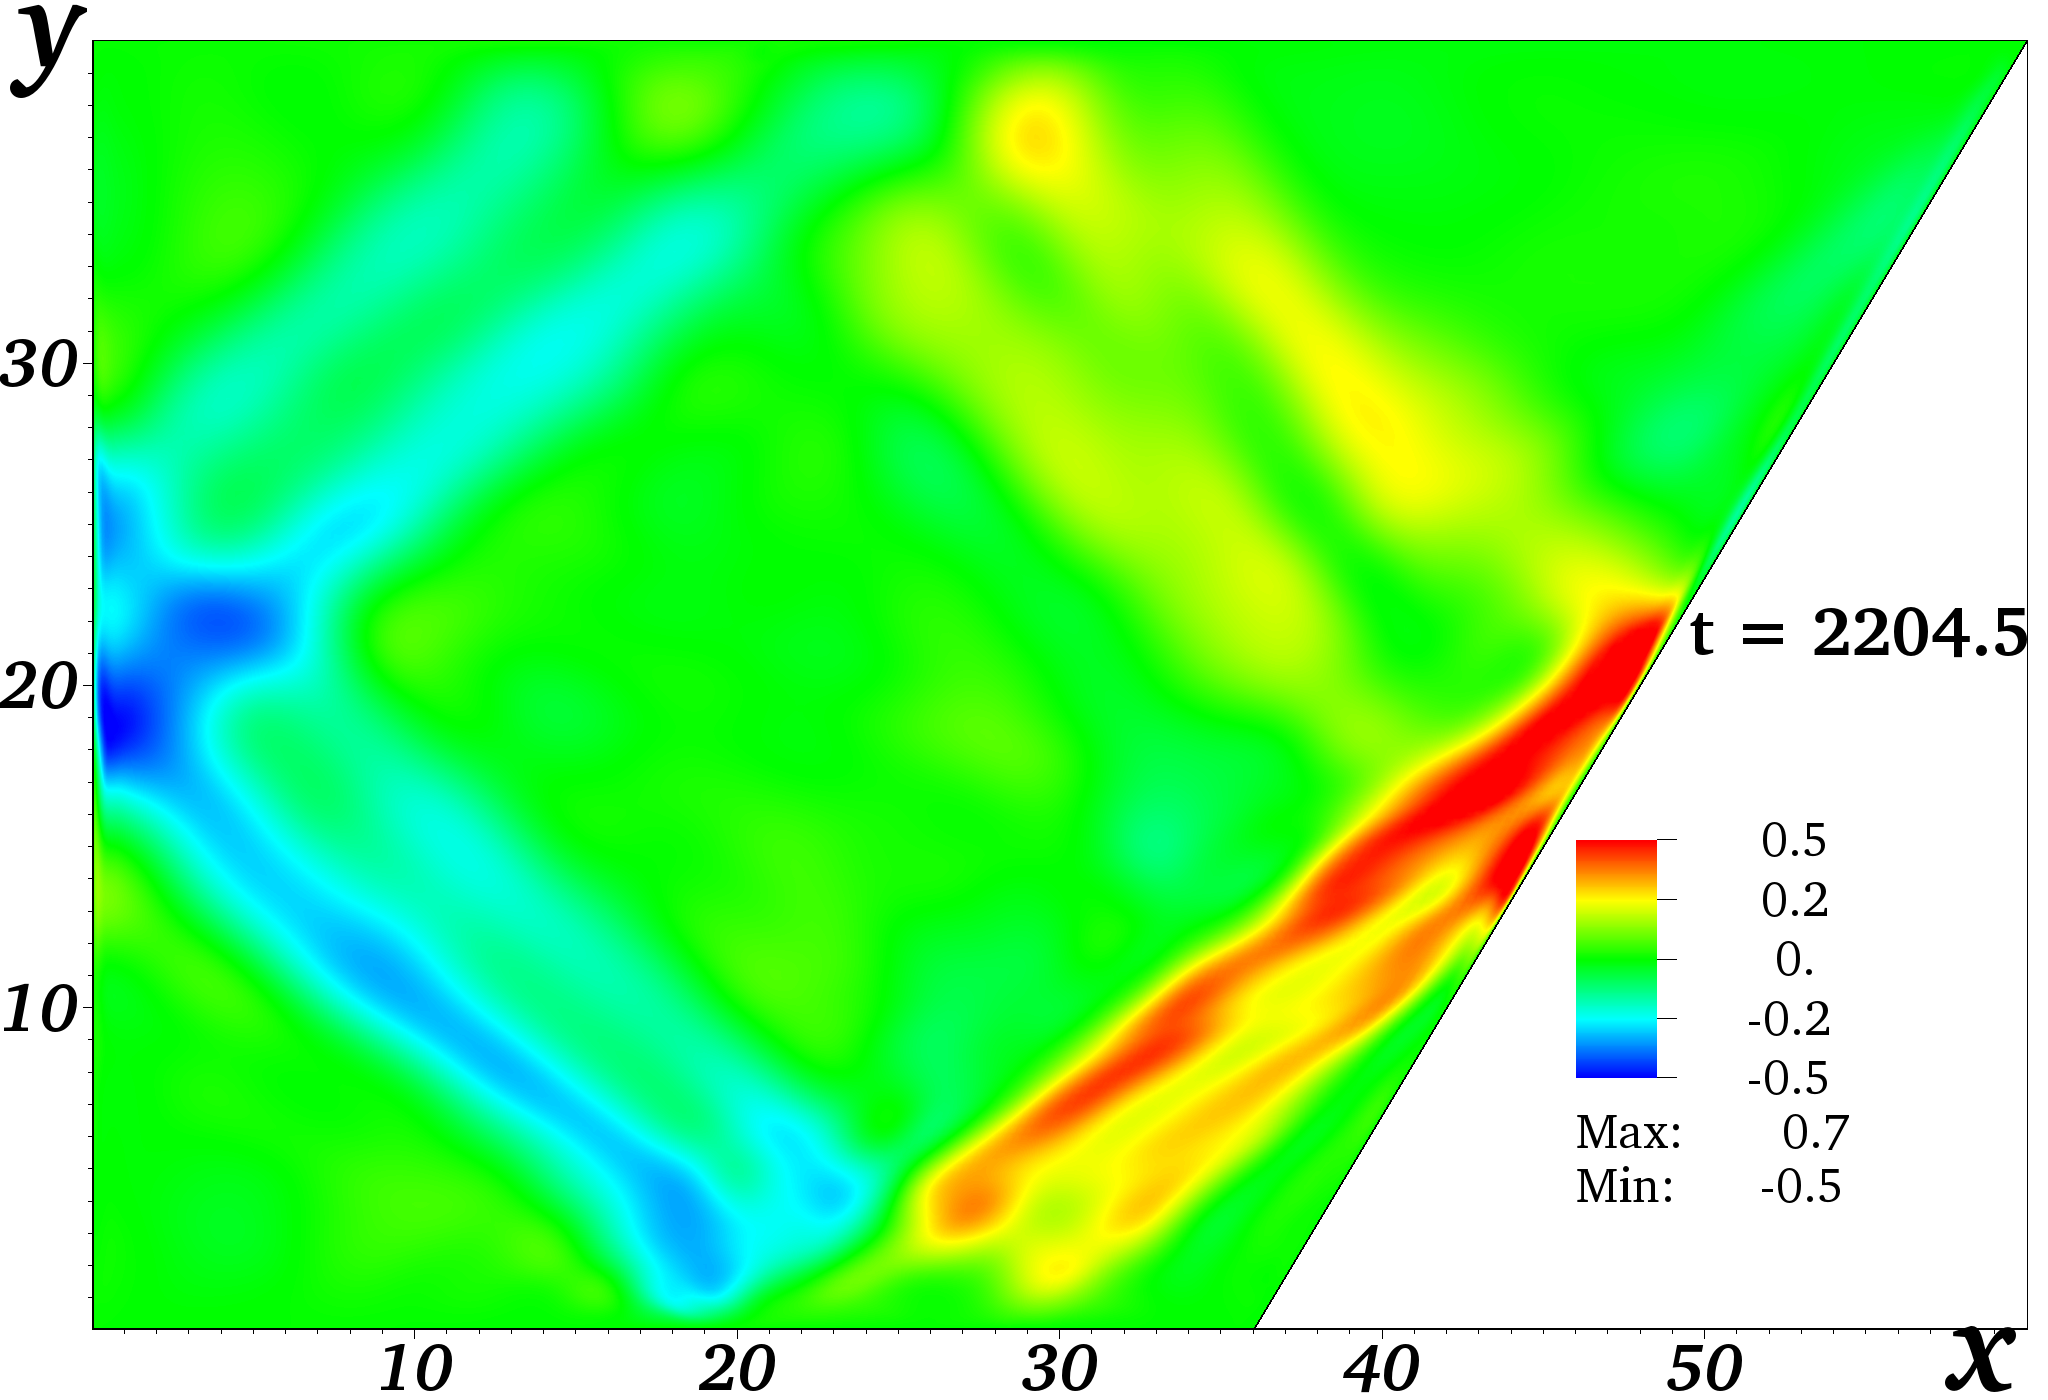
\includegraphics[width=1\textwidth]{pics/H40L60N1ap05dp20w1p63Deltawp05Biharm/2D36x36DiagramH40L60N1ap05dp20w0p63Deltawp3315BiharmVyn04408.png}
    \caption{Вертикальная компонента скорости при установлении аттрактора}
  \end{subfigure}
  \par
  \begin{subfigure}[с]{0.45\textwidth}
    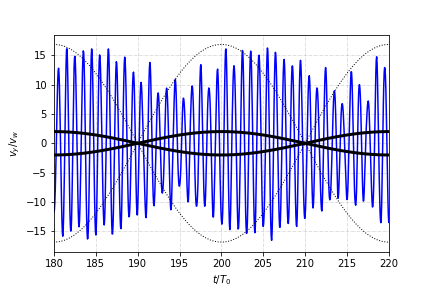
\includegraphics[width=1\textwidth]{pics/H40L60N1ap05dp20w1p63Deltawp05Biharm/vyX35p57Y11p27t4412.png}
    \caption{Вертикальная скорость}
  \end{subfigure}
  \begin{subfigure}[с]{0.45\textwidth}
    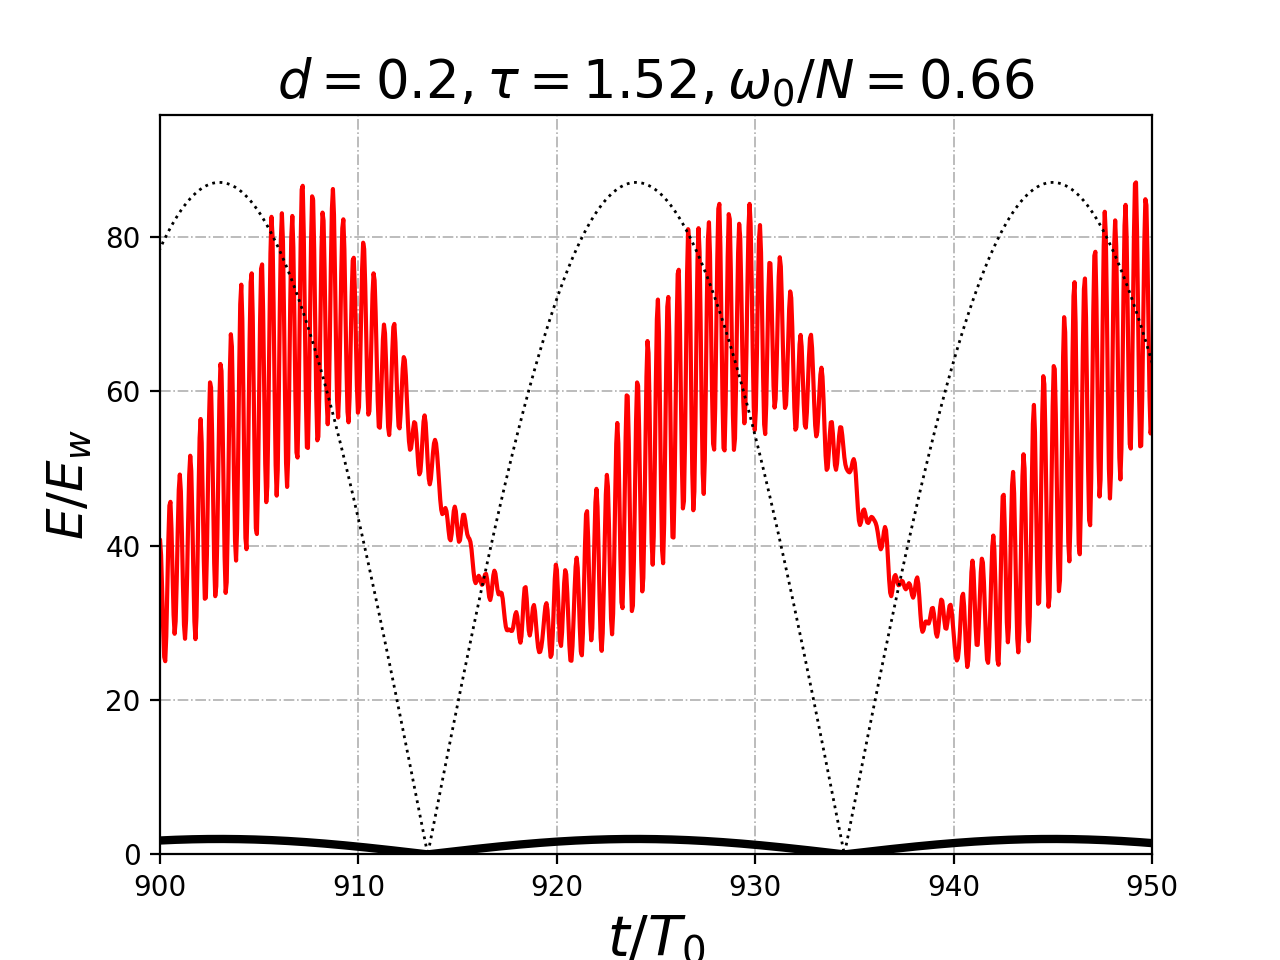
\includegraphics[width=1\textwidth]{pics/H40L60N1ap05dp20w1p63Deltawp05Biharm/2D36x36DiagramH40L60N1ap05dp20w1p63Deltawp05BiharmtotKEnonDim.png}
    \caption{Кинетическая энергия}
  \end{subfigure}
  \par
  \begin{subfigure}[с]{0.45\textwidth}
    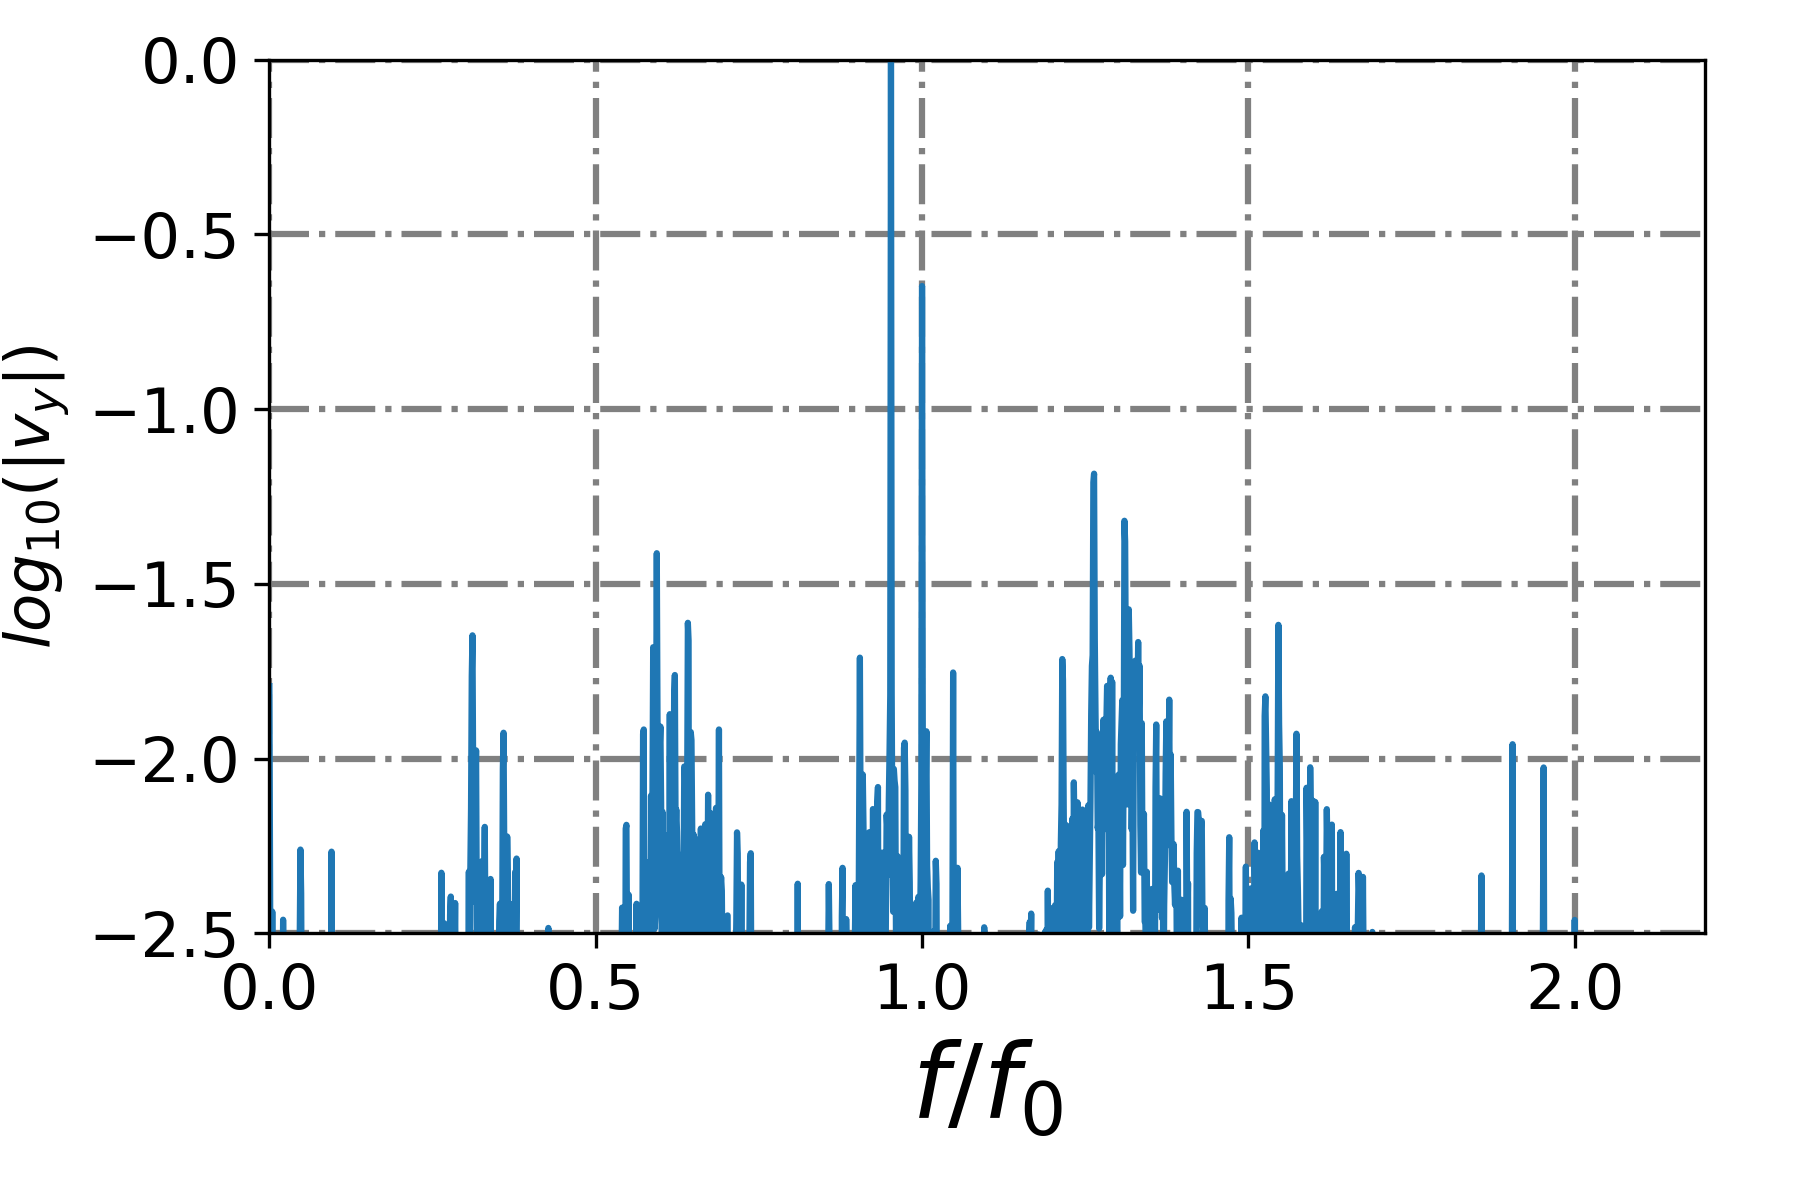
\includegraphics[width=1\textwidth]{pics/H40L60N1ap05dp20w1p63Deltawp05Biharm/spectrumX35p6Y11p2.png}
    \caption{Спектр}
  \end{subfigure}
  \begin{subfigure}[с]{0.45\textwidth}
    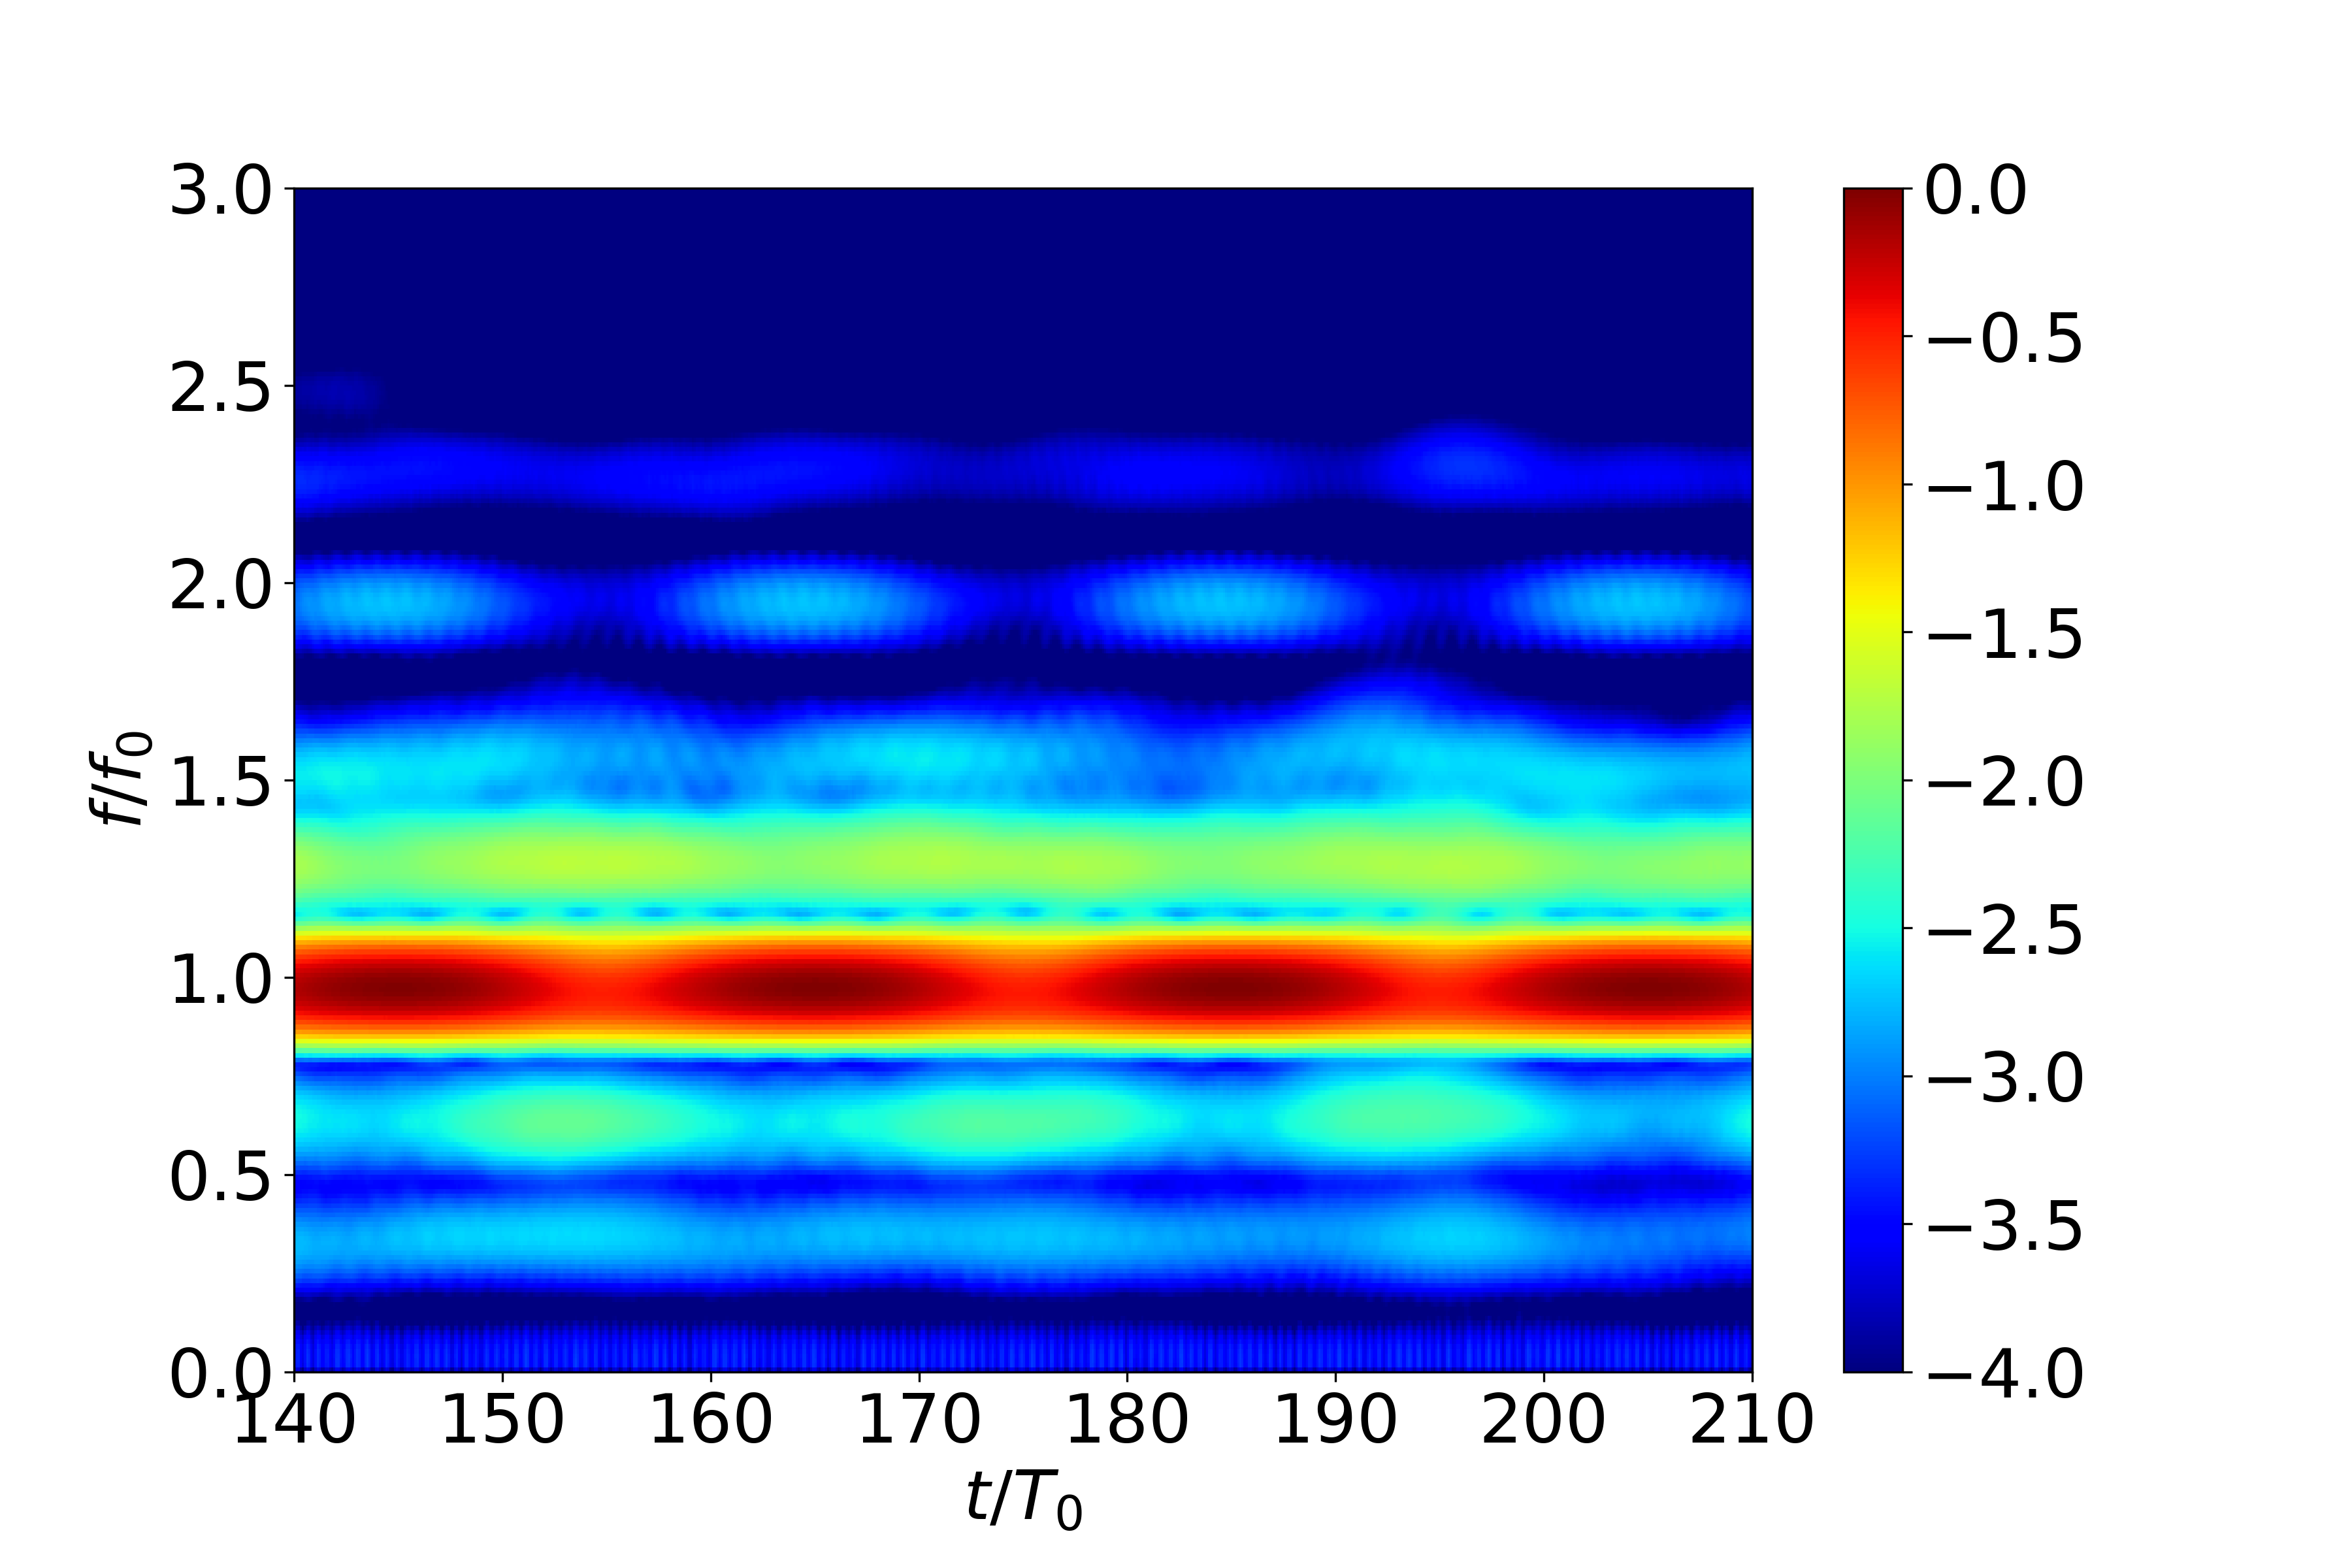
\includegraphics[width=1\textwidth]{pics/H40L60N1ap05dp20w1p63Deltawp05Biharm/TFspectrumX35p6Y11p2N200.png}
    \caption{Частотно-временная диаграмма}
    \label{}
  \end{subfigure}
  \caption{Результаты количественного исследования характеристик течения стратифицированной жидкости в трапециевидном резервуаре при внешнем воздействии с двумя приближенными частотами $\omega_1/N=0.66$ $\omega_2/N=0.68$. Черной линией  на графиках вертикальной скорости и кинетической энергии показана огибающая амплитуды колебаний волнпородуктора.}

  \label{fig:biharmVyap005-1}
\end{figure}

С приближением частот друг к другу(см. рис. \ref{fig:biharmVyap005-2}) появляются дополнительные дочерние волны, но режим успевает стабилизироваться во временной промежуток разности фаз двух частот. 

\begin{figure}
  \centering
  \begin{subfigure}[с]{0.45\textwidth}
    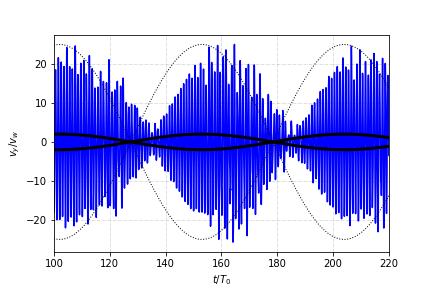
\includegraphics[width=1\textwidth]{pics/H40L60N1ap05dp20w1p63Deltawp02Biharm/vyX35p57Y11p27t4400.png}
    \caption{Вертикальная компонента скорости в зависимости от времени}
  \end{subfigure}
  \begin{subfigure}[с]{0.45\textwidth}
    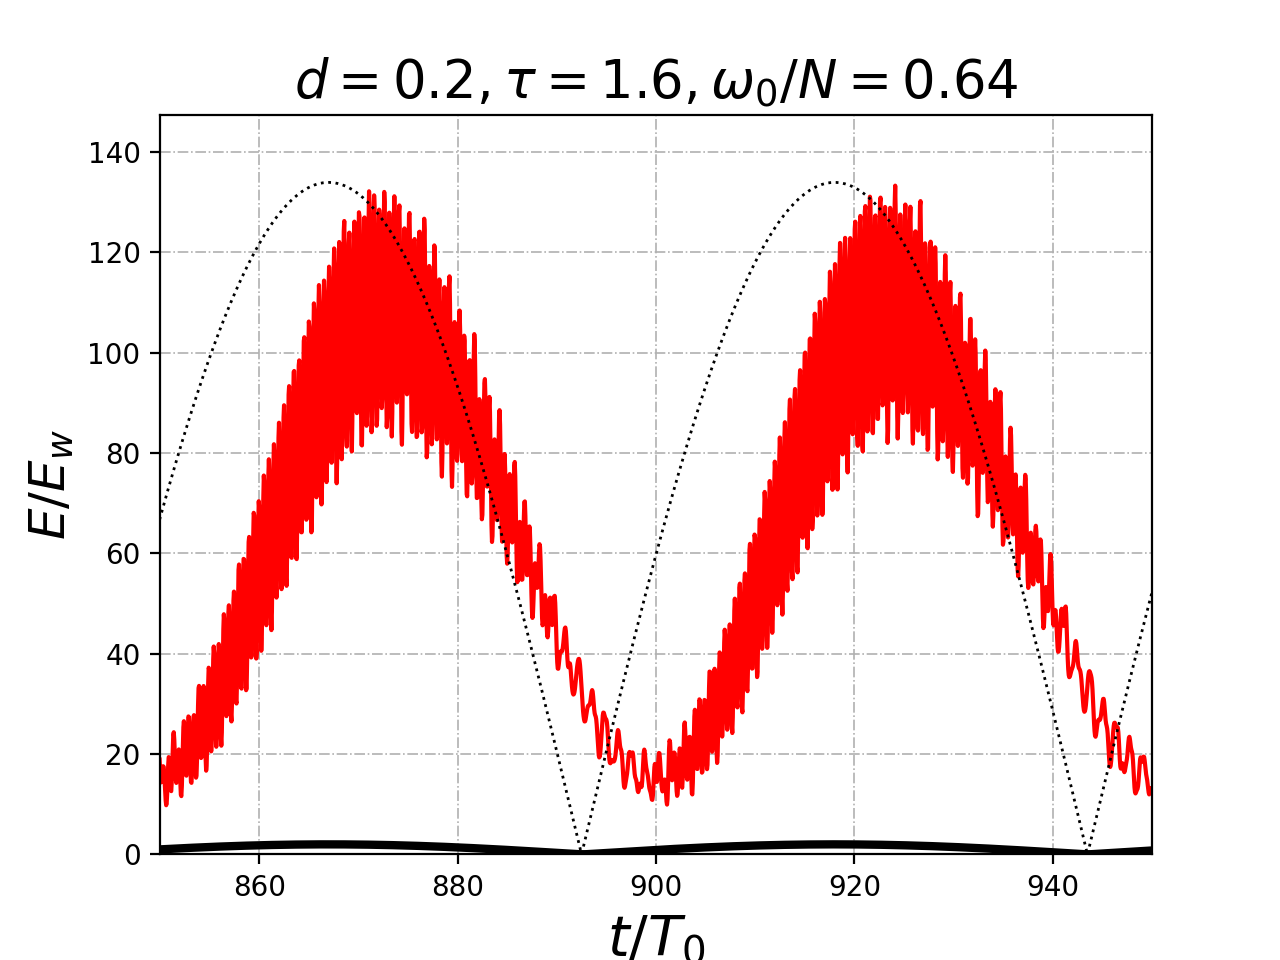
\includegraphics[width=1\textwidth]{pics/H40L60N1ap05dp20w1p63Deltawp02Biharm/2D36x36DiagramH40L60N1ap05dp20w1p63Deltawp02BiharmtotKEnonDim.png}
    \caption{Средняя кинетическая энергия в резервуаре в зависимости от времени}
  \end{subfigure}
  \par
  \begin{subfigure}[с]{0.45\textwidth}
    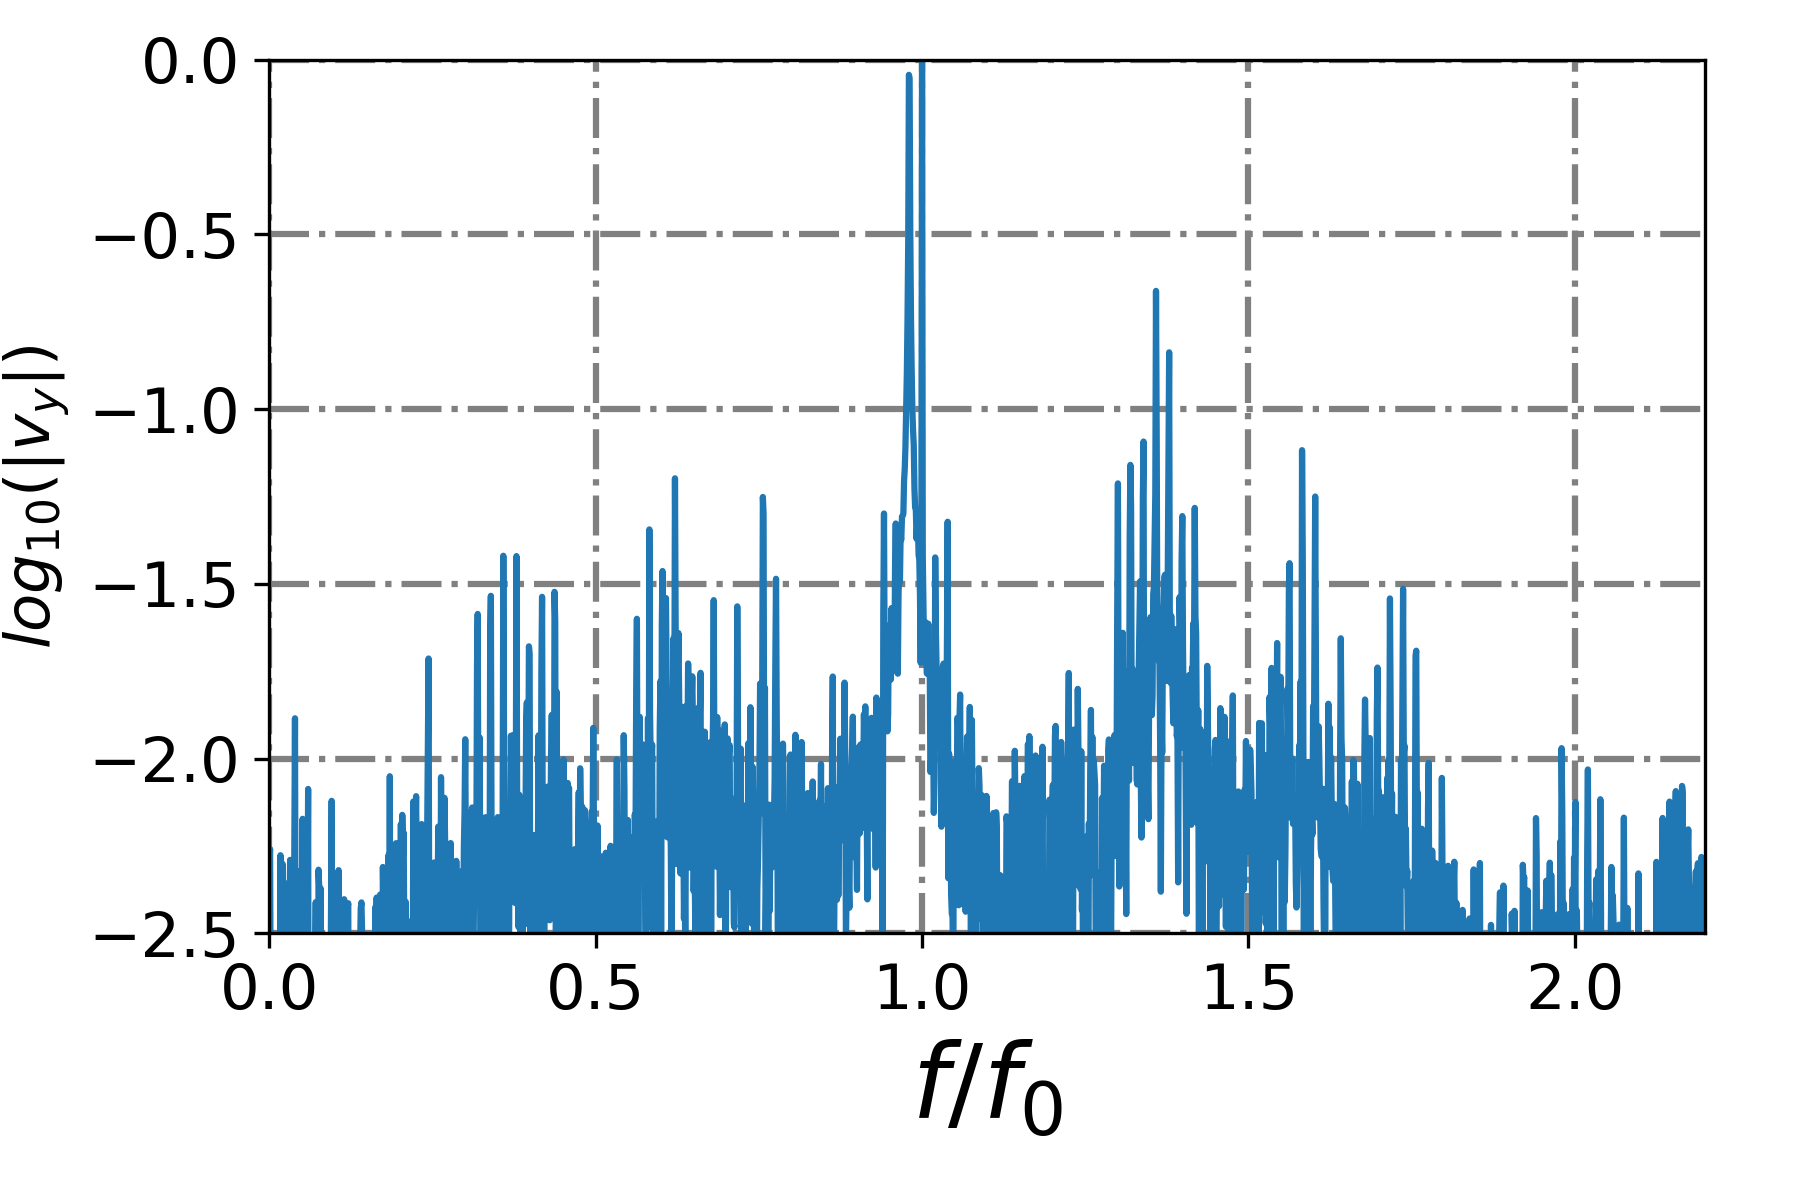
\includegraphics[width=1\textwidth]{pics/H40L60N1ap05dp20w1p63Deltawp02Biharm/spectrumX35p6Y11p2.png}
    \caption{Спектр}
  \end{subfigure}
  \begin{subfigure}[с]{0.45\textwidth}
    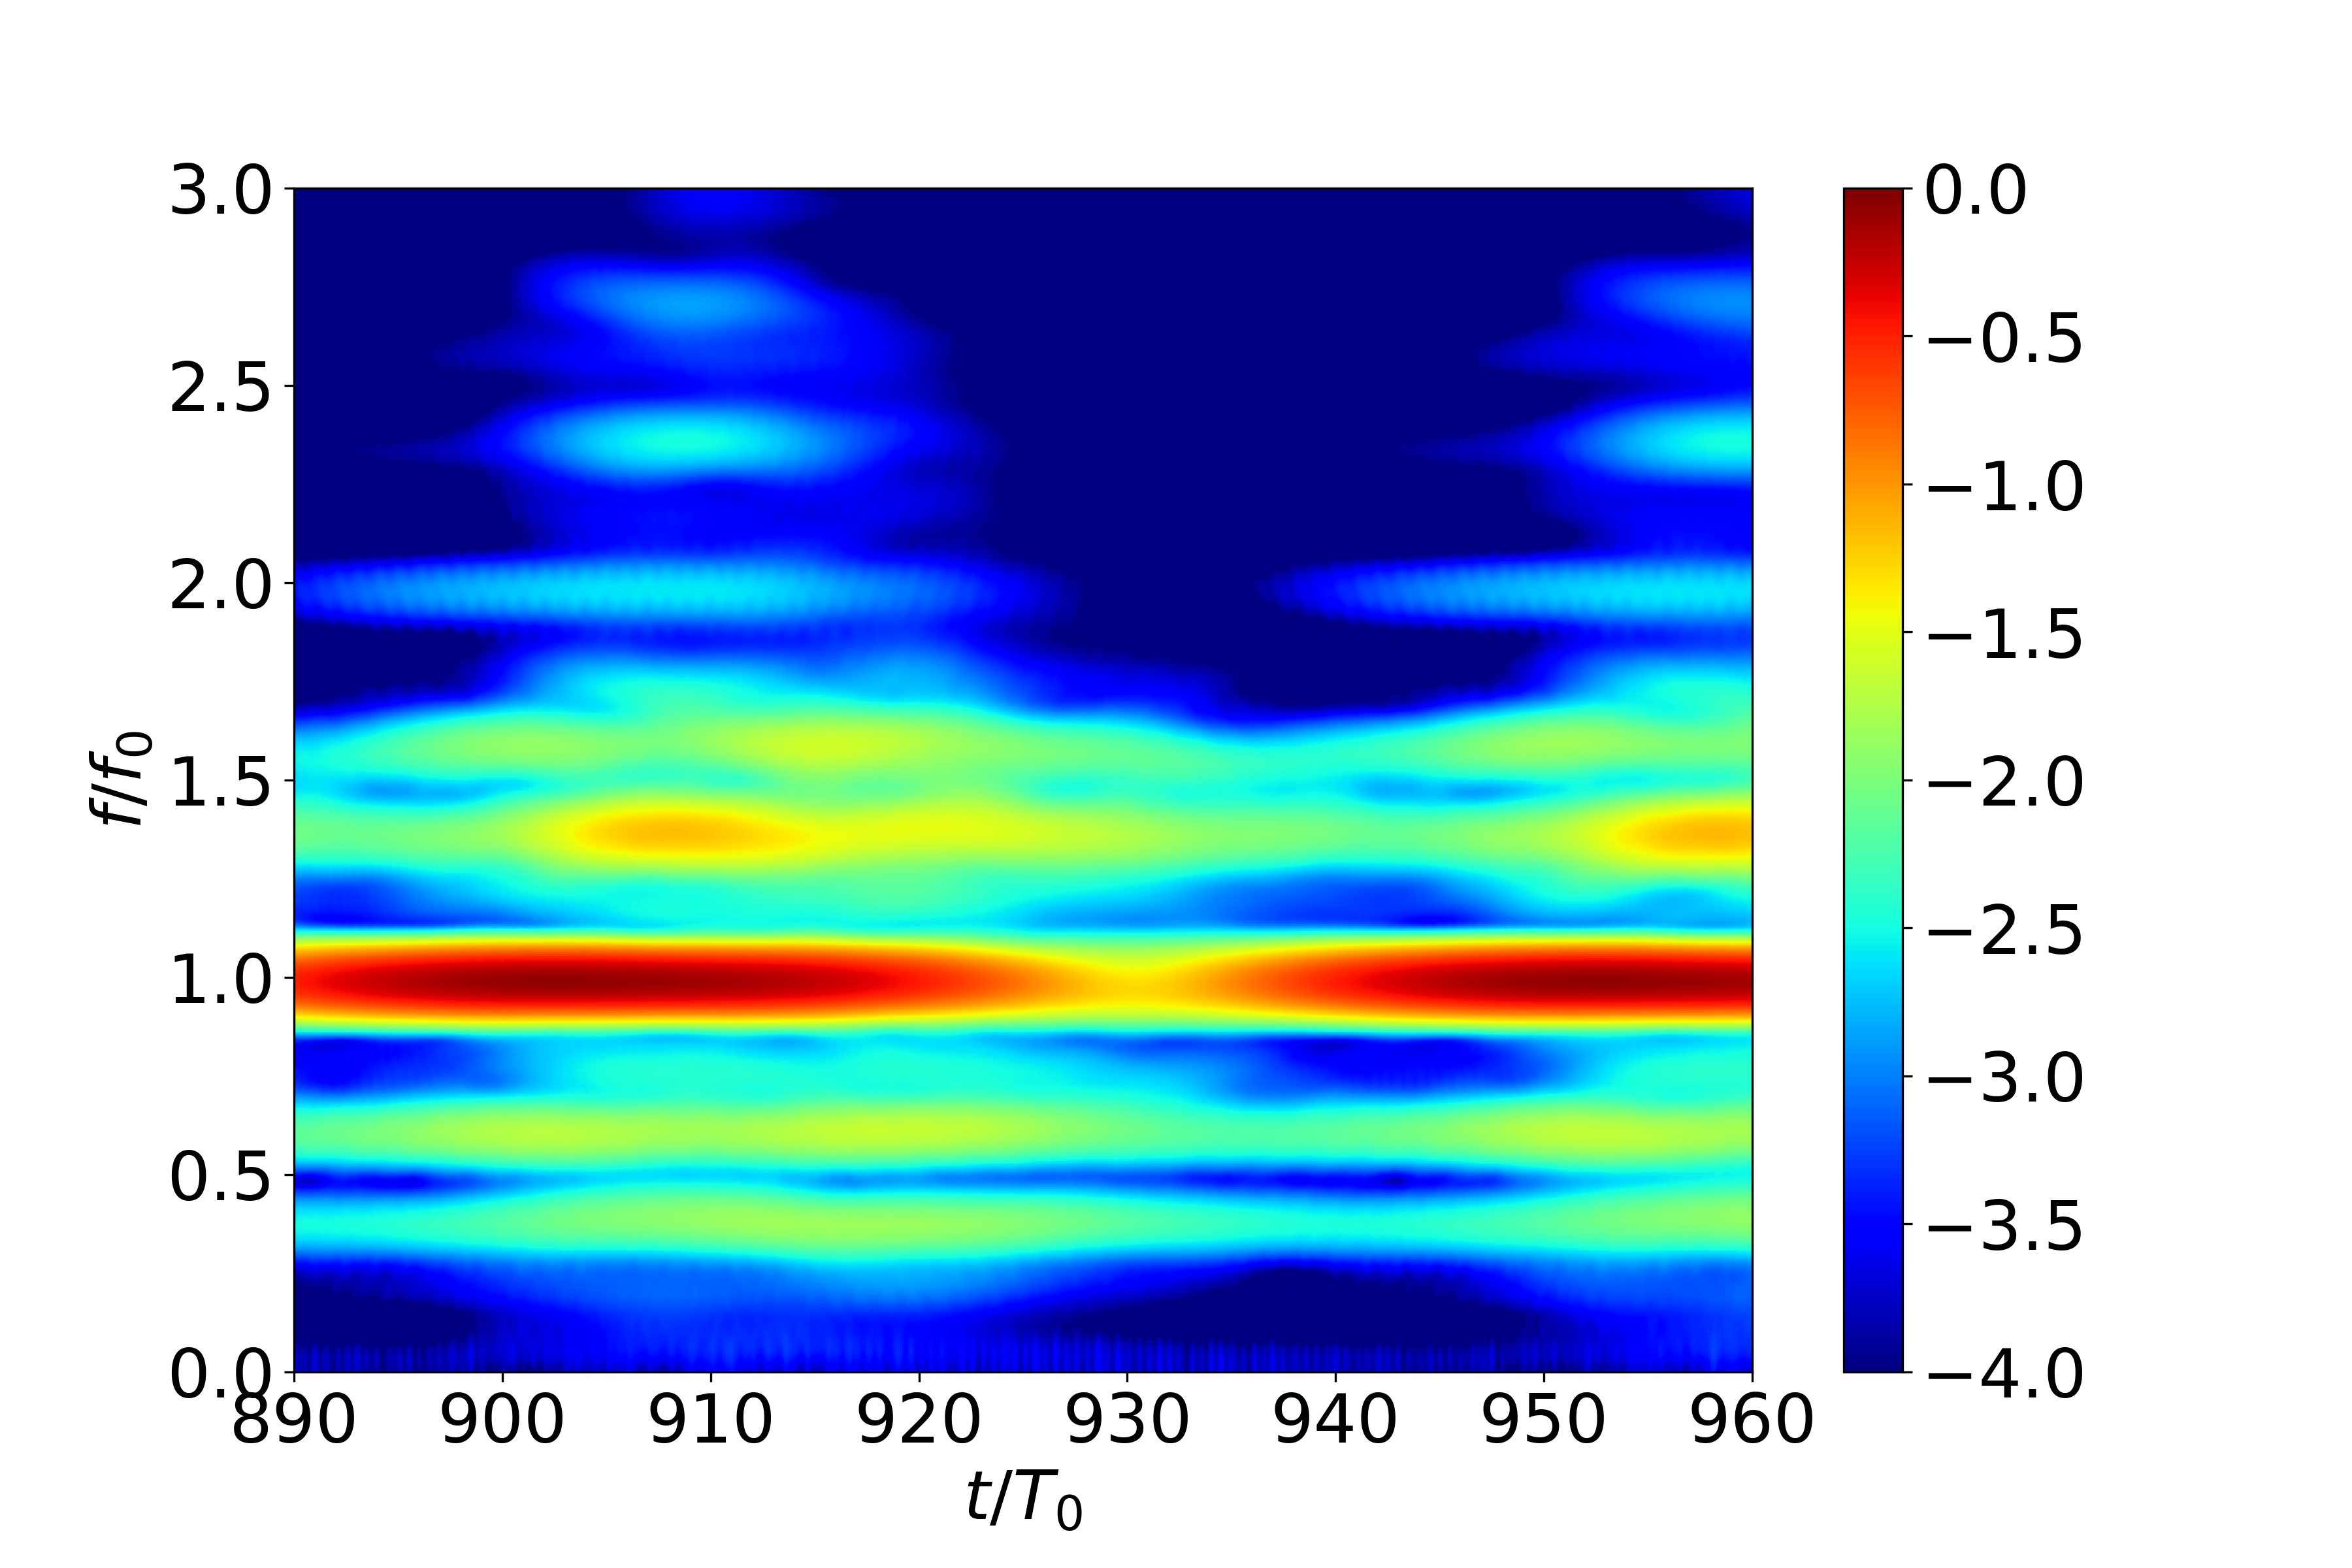
\includegraphics[width=1\textwidth]{pics/H40L60N1ap05dp20w1p63Deltawp02Biharm/TFspectrumX35p6Y11p2N256.png}
    \caption{Частотно-временная диаграмма}
  \end{subfigure}
  \caption{Количественные результаты исследования бигармонического аттрактора внутренних волн с двумя близкими частотами $\omega_1/N=0.628$,  $\omega_2/N=0.641$.}
  \label{fig:biharmVyap005-2}
\end{figure}

Помимо детального анализа результатов моделирования бигармонических аттракторов полученных с помощью метода спектральных элементов, были получены результаты моделирования с помощью метода конечного объема (см. рис. \ref{fig:biharm}). Из рисунка видно, что качественно картина течения совпала с предсказанной при помощи трассировки лучей. 

\begin{figure}
    \centering
    \scalebox{0.95}{
    \begin{tikzpicture}[scale=1.187, z={(-.707,-.5)}]
        \node[anchor=south west,inner sep=0] at (0,0) {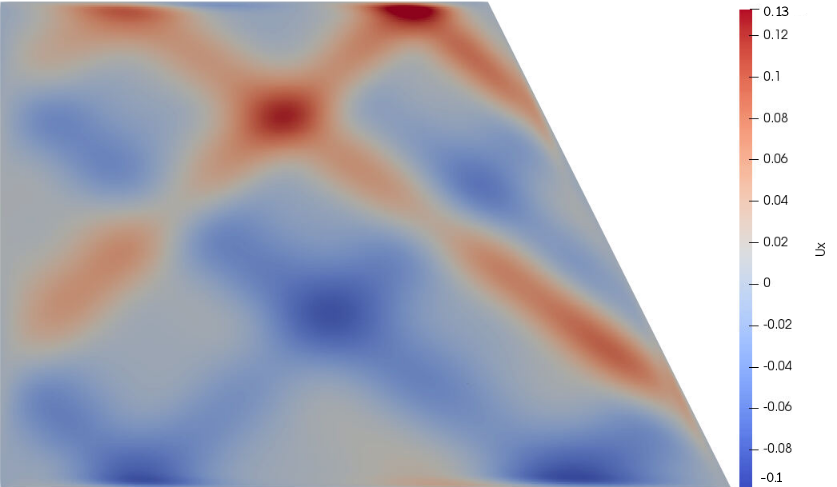
\includegraphics[width=\textwidth]{pics/Biharm.png}};
        \draw (0,0,0) -- (12*0.98,0,0) -- (8*0.98,8*0.98,0)--(0,8*0.98,0) --cycle;
        \draw[style = dashed] (9*0.98,0,0)   -- (0,6.4*0.98,0) -- (2.0*0.98,8*0.98,0) -- (5.65*2*0.98,1.4*0.98,0)-- cycle;
        \draw[style = dashed] (0,0.985*2*0.98,0) -- (6.6*0.98,8*0.98,0) -- (9*0.98,6*0.98,0) -- (2.2*0.98,0,0)  -- cycle;
        \draw[thick,->] (9,6,0) -- (11.1,6,0) node[anchor=north east]{$x$};
        \draw[thick,->] (9,6,0) -- (9.1,8,0) node[anchor=north west]{$z$};
    \end{tikzpicture}
    }
    \caption{Поле горизонтальной компоненты скорости для бигармонического аттрактора и трассировка лучей.}
    \label{fig:biharm}
\end{figure}


\section{Кинетическая энергия для монохроматического и бигармонического режимов}

 Для геометрии, показанной на рис.\ref{fig:domainup}, нижняя и верхняя границы диапазона существования аттрактора соответствуют $\omega_{cr1}/N=0.55$ и $\omega_{cr2}/N=0.74$. При достижении этих критических значений частот происходит вырождение параллелограмма в диагональ трапеции. В качестве интегральной размерной меры эффективности генерации аттрактора при постоянной амплитуде волнопродуктора и неизменной форме резервуара принята кинетическая энергия жидкости, проинтегрированная по площади трапеции $S$: $E_{k}(t)=\int_{S}\frac{\rho_{m}}{2}\left[v_{y}^2(t)+v_{x}^2(t)\right]dS$. Для этой меры можно ввести значение, осредненное в скользящем временном окне по достаточно большому числу периодов колебаний $<E_{k}(t)>$, и вариацию относительно среднего, рассчитываемую как $r=D(E_{k}(t)-<E_{k}(t)>)/<E_{k}(t)>$, где $D(E_{k}(t)-<E_{k}(t)>)$ -- дисперсия относительно среднего. Безразмерные величины $\overline{E}_{k}(t)$ и $<\overline{E}_{k}(t)>$ определены путем нормировки на величину $\rho_{m}S(a\omega)^2/2$. Известно, что режимы движения в аттракторах могут быть близки как к прогрессивным, так и к стоячим волнам ~\cite{Brouzetetal2017}. Величина $r$ позволяет дать количественную оценку близости наблюдаемого режима к одному из этих предельных случаев \cite{Brouzetetal2017}. 


Характерный вид зависимостей, наблюдаемых в монохроматическом режиме при малой амплитуде колебаний показан на 

рис. \ref{fig:domainup}
для  $a=0.02$cм ($a/H=5\cdot 10^{-4}$), $\omega/N=0.63$. Характерное время выхода системы на установившийся режим составляет порядка $30$ периодов колебаний, спектр сигнала является с высокой точностью монохроматическим, колебания кинетической энергии относительно среднего имеют небольшую амплитуду ($r=0.103$). За первую ветвь аттрактора принят пучок с наибольшим значением плотности энергии, возникающий после фокусирующего отражения от наклонной стенки. Величины интегральных параметров, характеризующих линейные монохроматические режимы при фиксированном значении $a/H=5\cdot 10^{-4}$ в частотном диапазоне от $\omega_{cr1}/N=0.55$ до $\omega_{cr2}/N=0.74$ приведены в таблице \ref{tab:bolts002}. Видно, что при фиксированной амплитуде колебаний величина кинетической энергии аттрактора максимальна при $\omega/N=0.63$. Очевидно, что при этом значении частоты возмущающего воздействия следует ожидать сильных нелинейных эффектов при увеличении амплитуды колебаний волнопродуктора. Величина $r$ при $\omega/N=0.63$ достигает минимума: движение в аттракторе представлено прогрессивной волной.  Характерные картины течения и зависимости, наблюдаемые в случае слабонелинейного режима при $\omega/N=0.63$ приведены на рис.\ref{fig:Vyamp05} для $a=0.05$см ($a/H=1.25\cdot 10^{-3}$). В слабонелинейном режиме имеет место триадный резонанс \cite{Dauxoisetal2018}, при котором генерируются две дочерние субгармонические волны малой амплитуды.  Частотно-временная диаграмма, показанная на рис. \ref{fig:Vyamp05}, представляет собой спектр сигнала, вычисленный в скользящем окне и осредненный по окрестности точки, лежащей в середине первой ветви аттрактора. Частотный спектр внутренних волн при данном режиме является дискретным, с доминирующим вкладом, соответствующим частоте возмущения $\omega_{0}$, двумя дочерними субгармоническими частотами $\omega_{1}^{*}+\omega_{2}^{*}=\omega_{0}$, двумя супергармоническими частотам $\omega_{1}^{**}=\omega_{1}^{*}+\omega_{0}$, $\omega_{2}^{**}=\omega_{2}^{*}+\omega_{0}$ и удвоенной частотой $2\omega_{0}$. 


\begin{figure}
	\centering
	\begin{subfigure}[с]{0.45\textwidth}
	    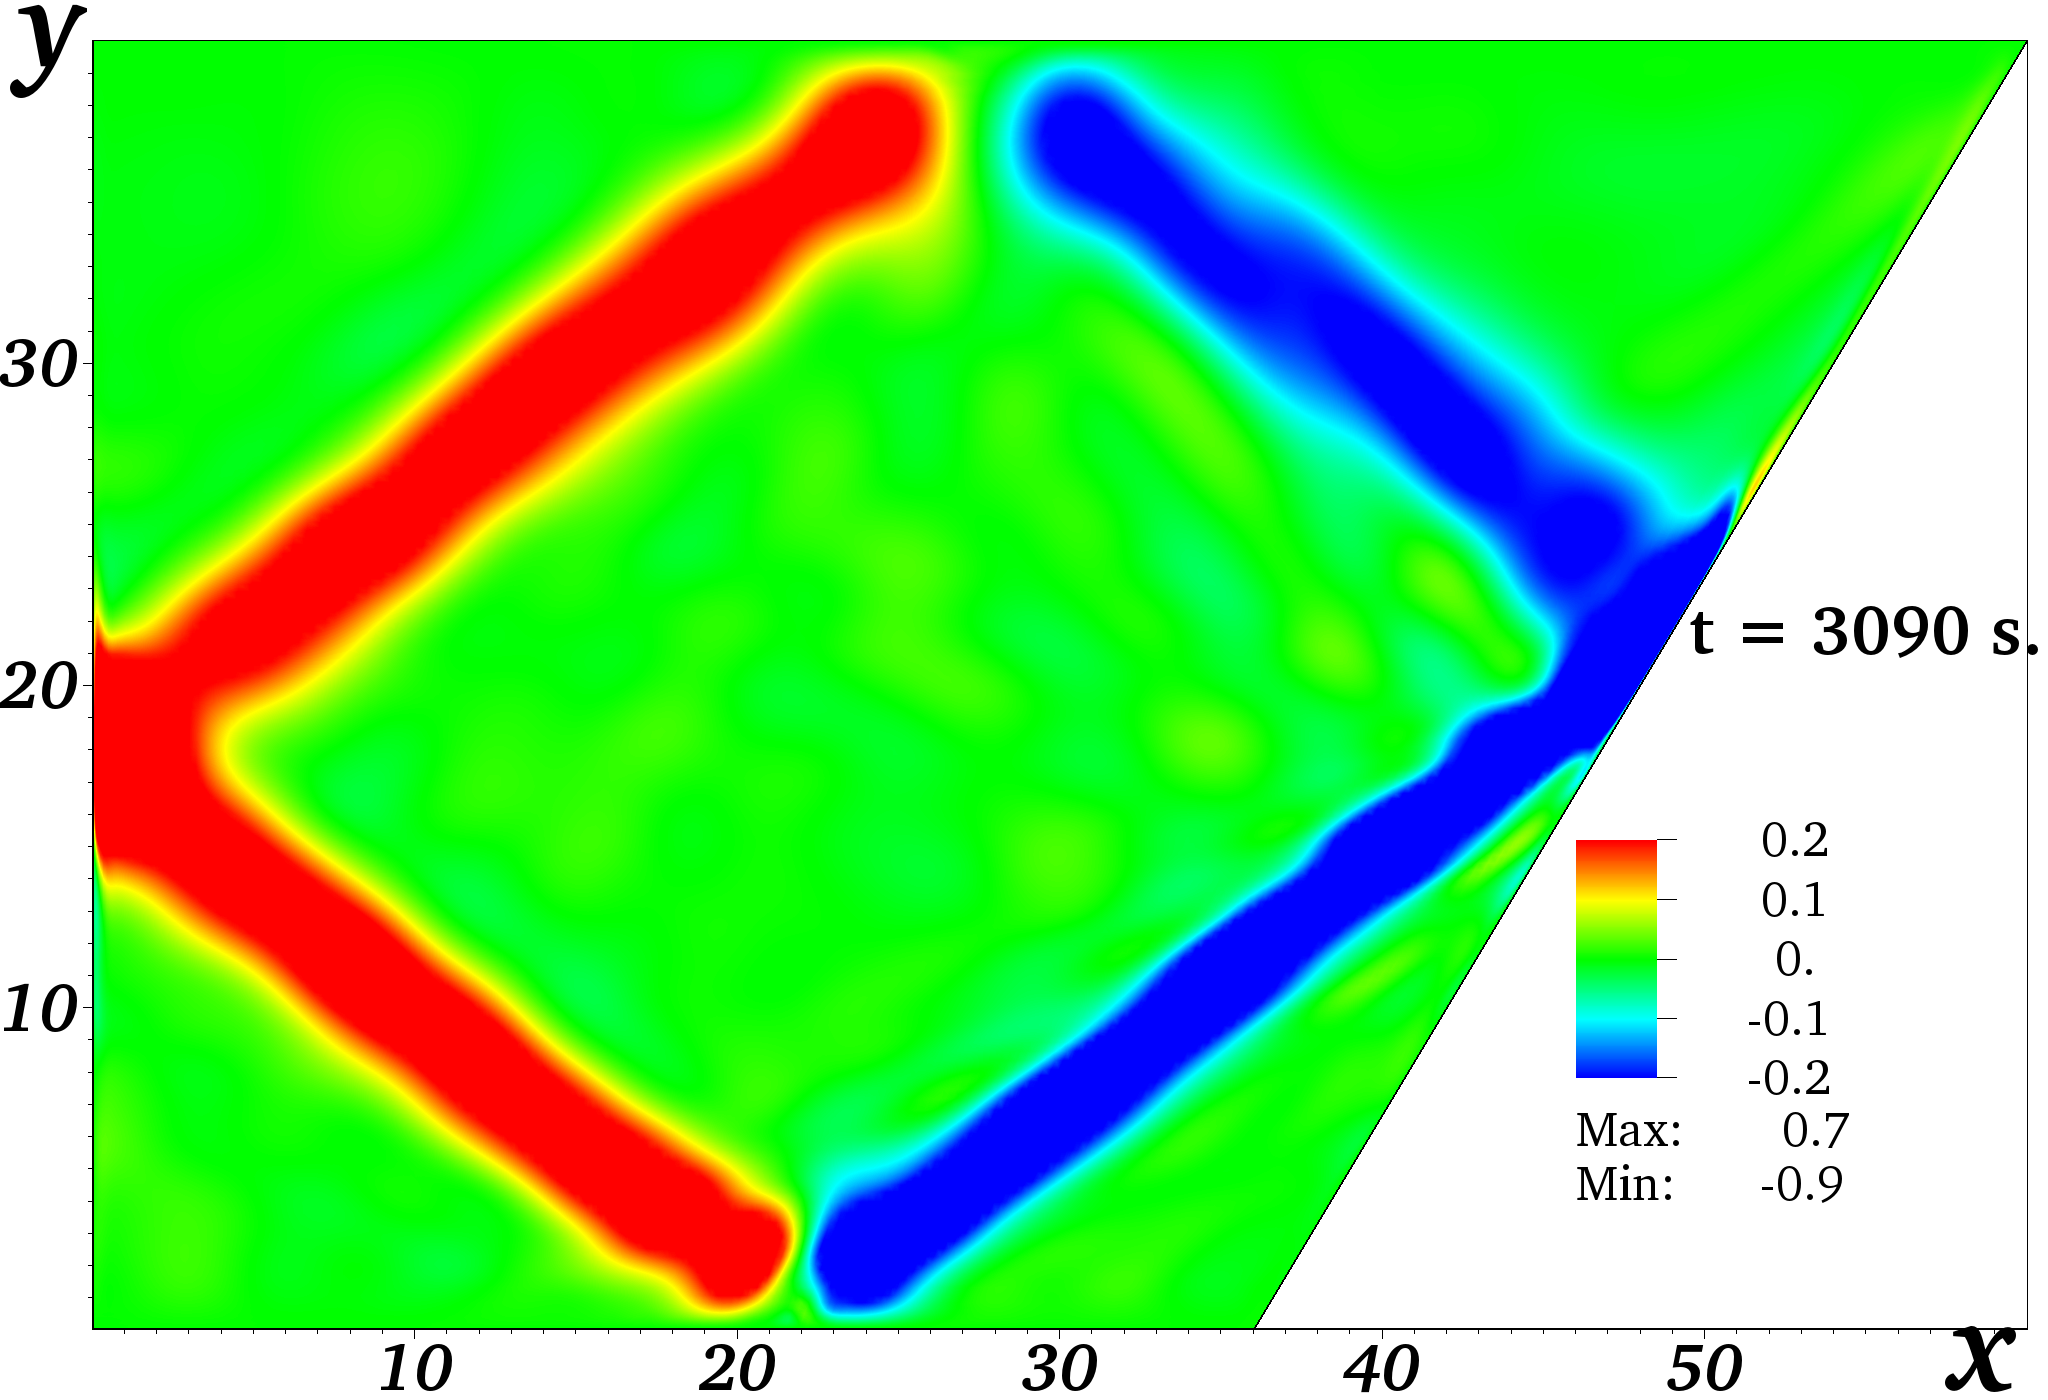
\includegraphics[width=1\textwidth]{pics/H40L60N1ap05dp20w0p63/2D36x36DiagramH40L60N1ap05dp20w0p63Vyn00308.png}
	    \caption{Поле вертикальной компоненты скорости при монохроматическом внешнем воздействии с амплитудой($a/H=5\cdot 10^{-4}$)}
	\end{subfigure}
	\begin{subfigure}[с]{0.45\textwidth}
	    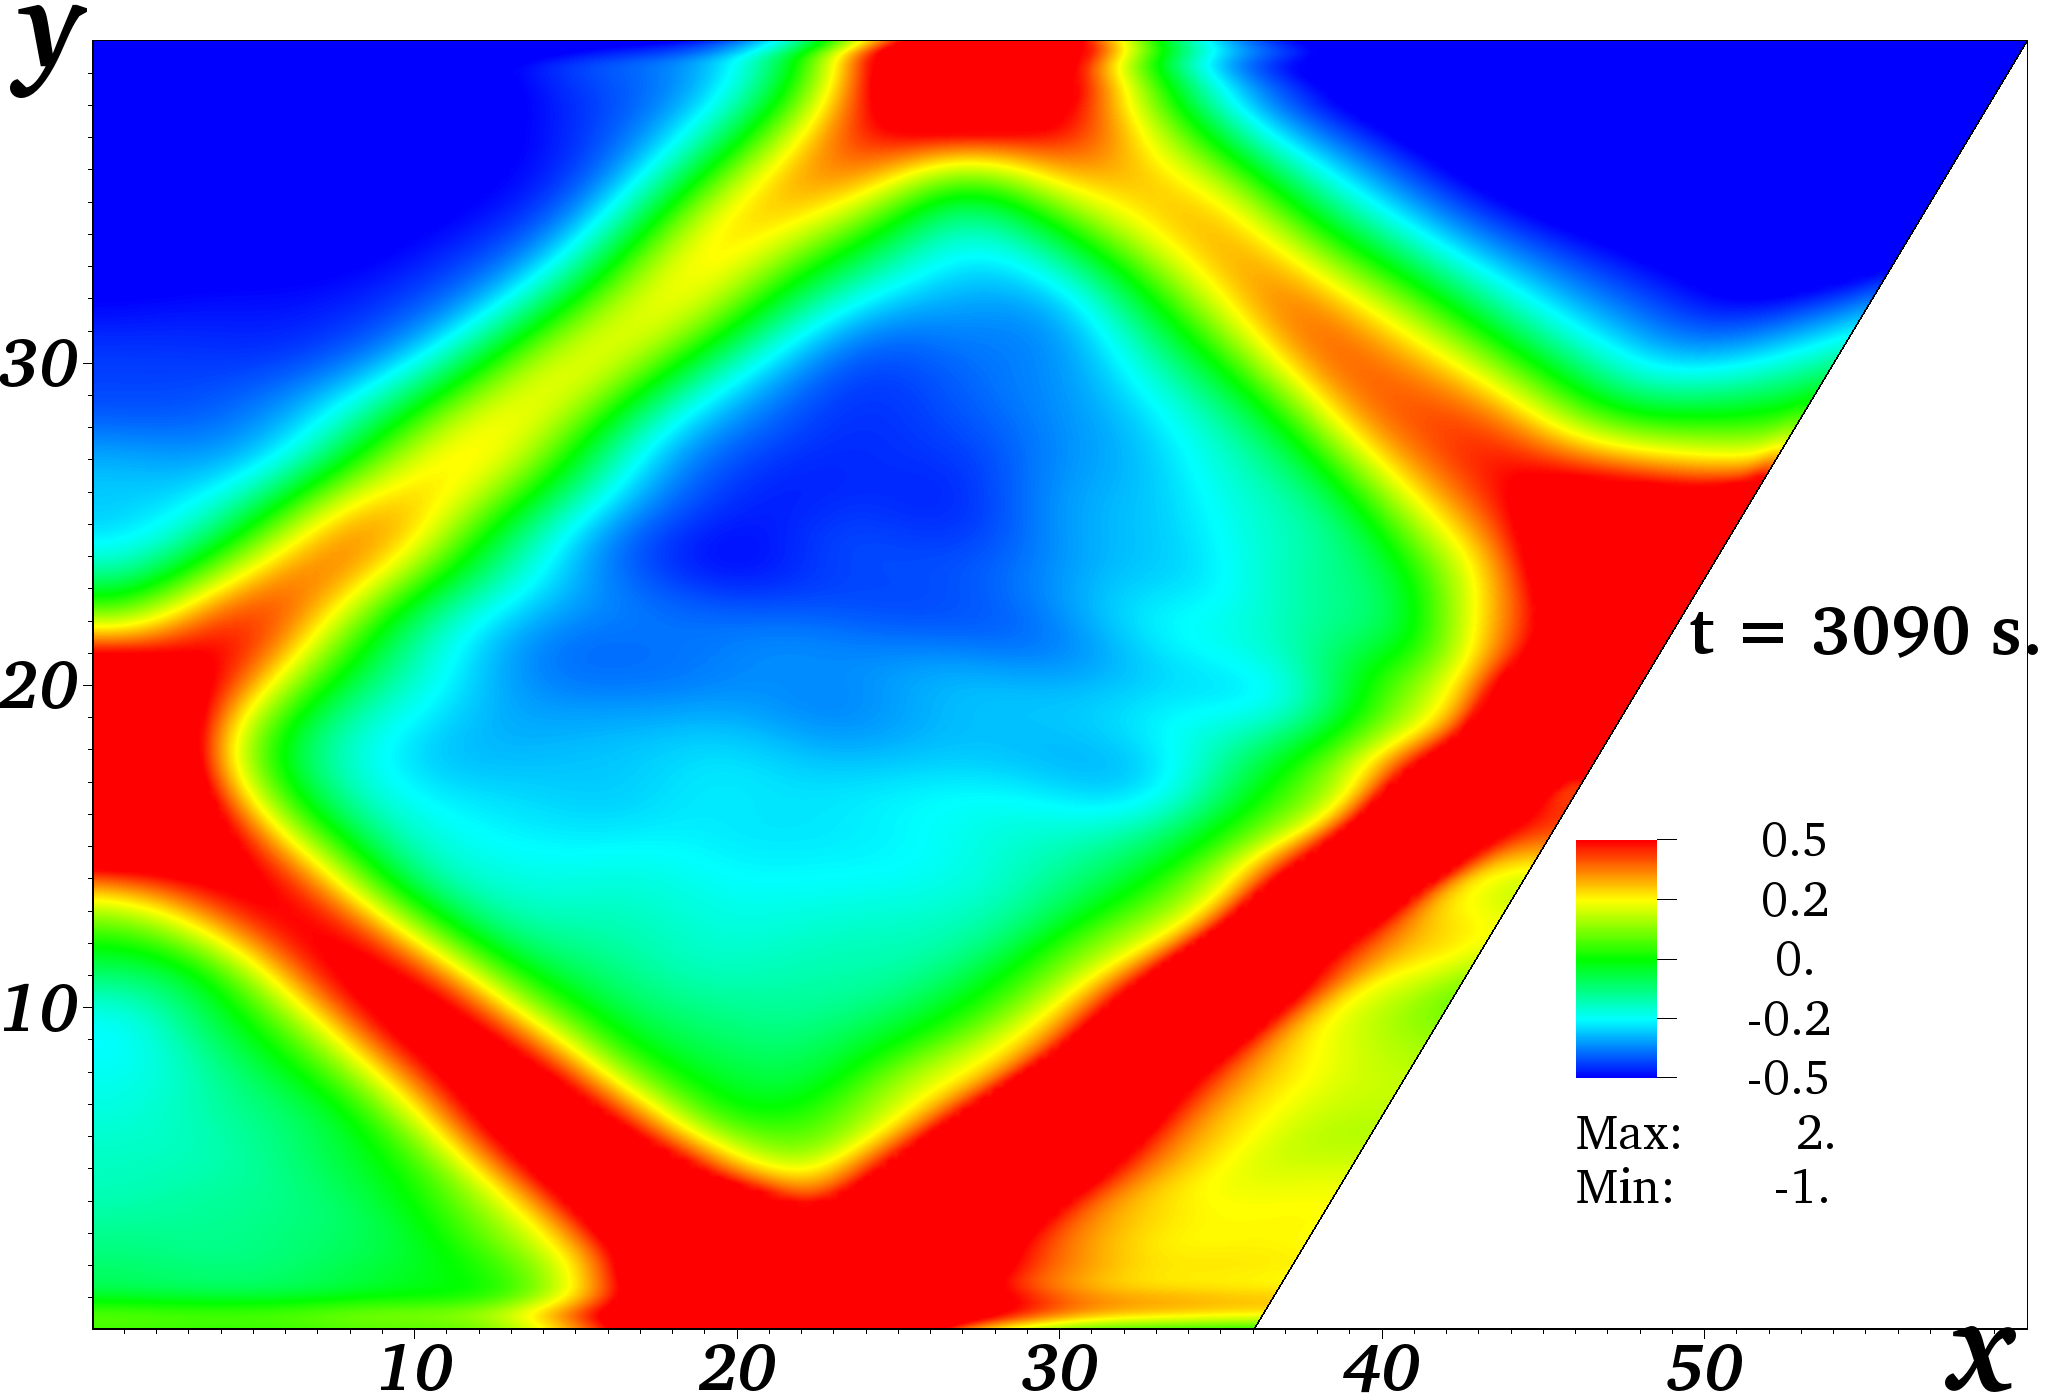
\includegraphics[width=1\textwidth]{pics/H40L60N1ap05dp20w0p63/2D36x36DiagramH40L60N1ap05dp20w0p63Pn00308.png}
	    \caption{Поле давления при монохроматическом внешнем воздействии с амплитудой ($a/H=5\cdot 10^{-4}$)}
	\end{subfigure}
	\par
	\begin{subfigure}[с]{0.45\textwidth}
	    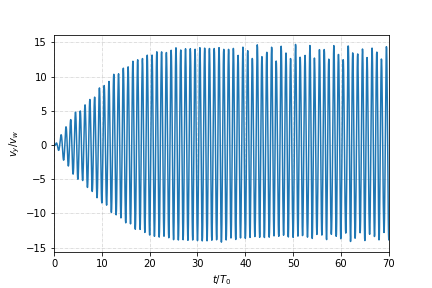
\includegraphics[width=1\textwidth]{pics/H40L60N1ap05dp20w0p63/vyX35p57Y11p27t4400.png}
	    \caption{Скорость в середине первого луча аттрактора}
	\end{subfigure}
	\begin{subfigure}[с]{0.45\textwidth}
	    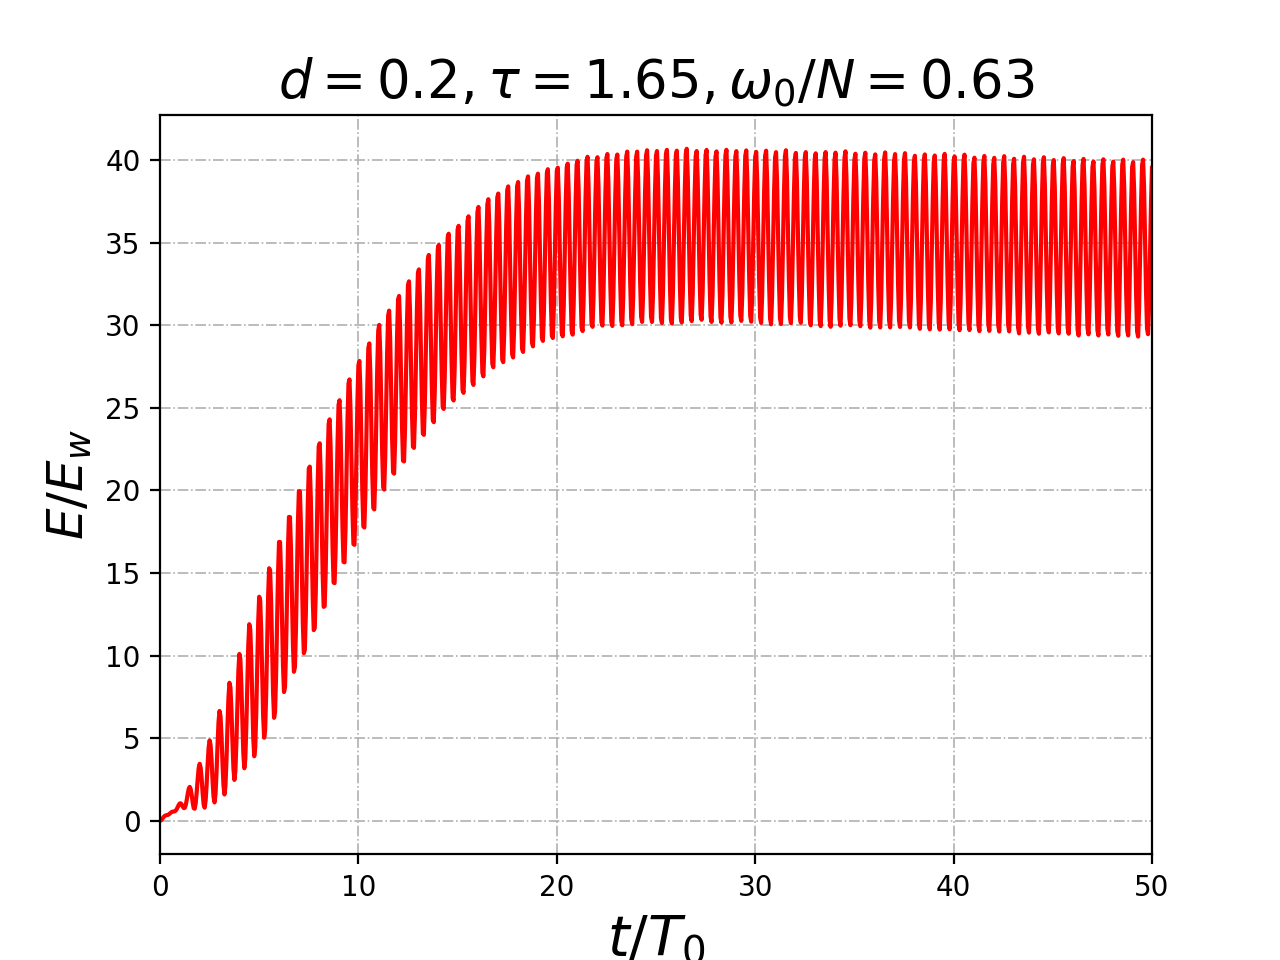
\includegraphics[width=1\textwidth] {pics/H40L60N1ap05dp20w0p63/2D36x36DiagramH40L60N1ap05dp20w0p63totKEnonDim.png}
	    \caption{Кинетическая энергия в середине первого луча аттрактора}
	\end{subfigure}
	\par
	\begin{subfigure}[с]{0.45\textwidth}
	    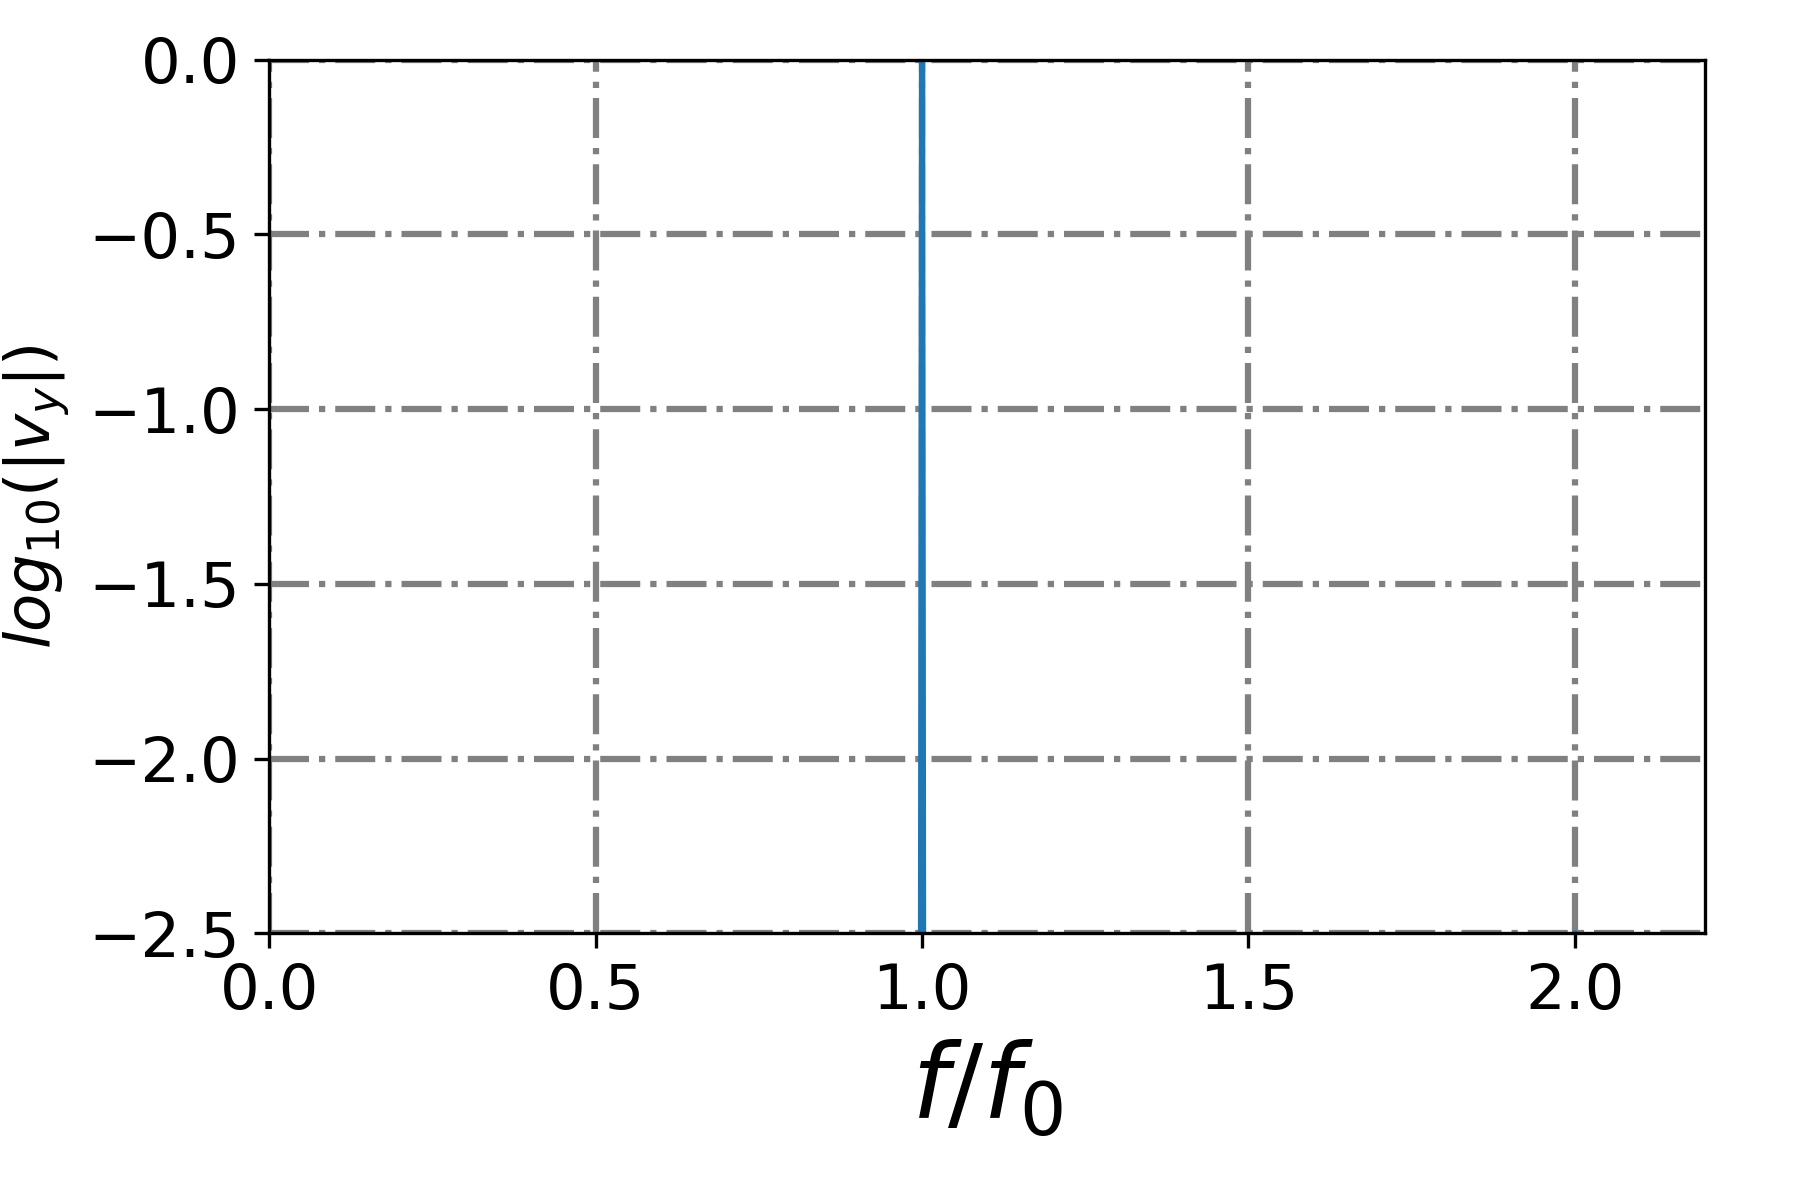
\includegraphics[width=1\textwidth]{{pics/H40L60N1ap05dp20w0p63/spectrumX35.6Y11.2}.png}
	    \caption{Спектр}
	\end{subfigure}
	\begin{subfigure}[с]{0.45\textwidth}
	    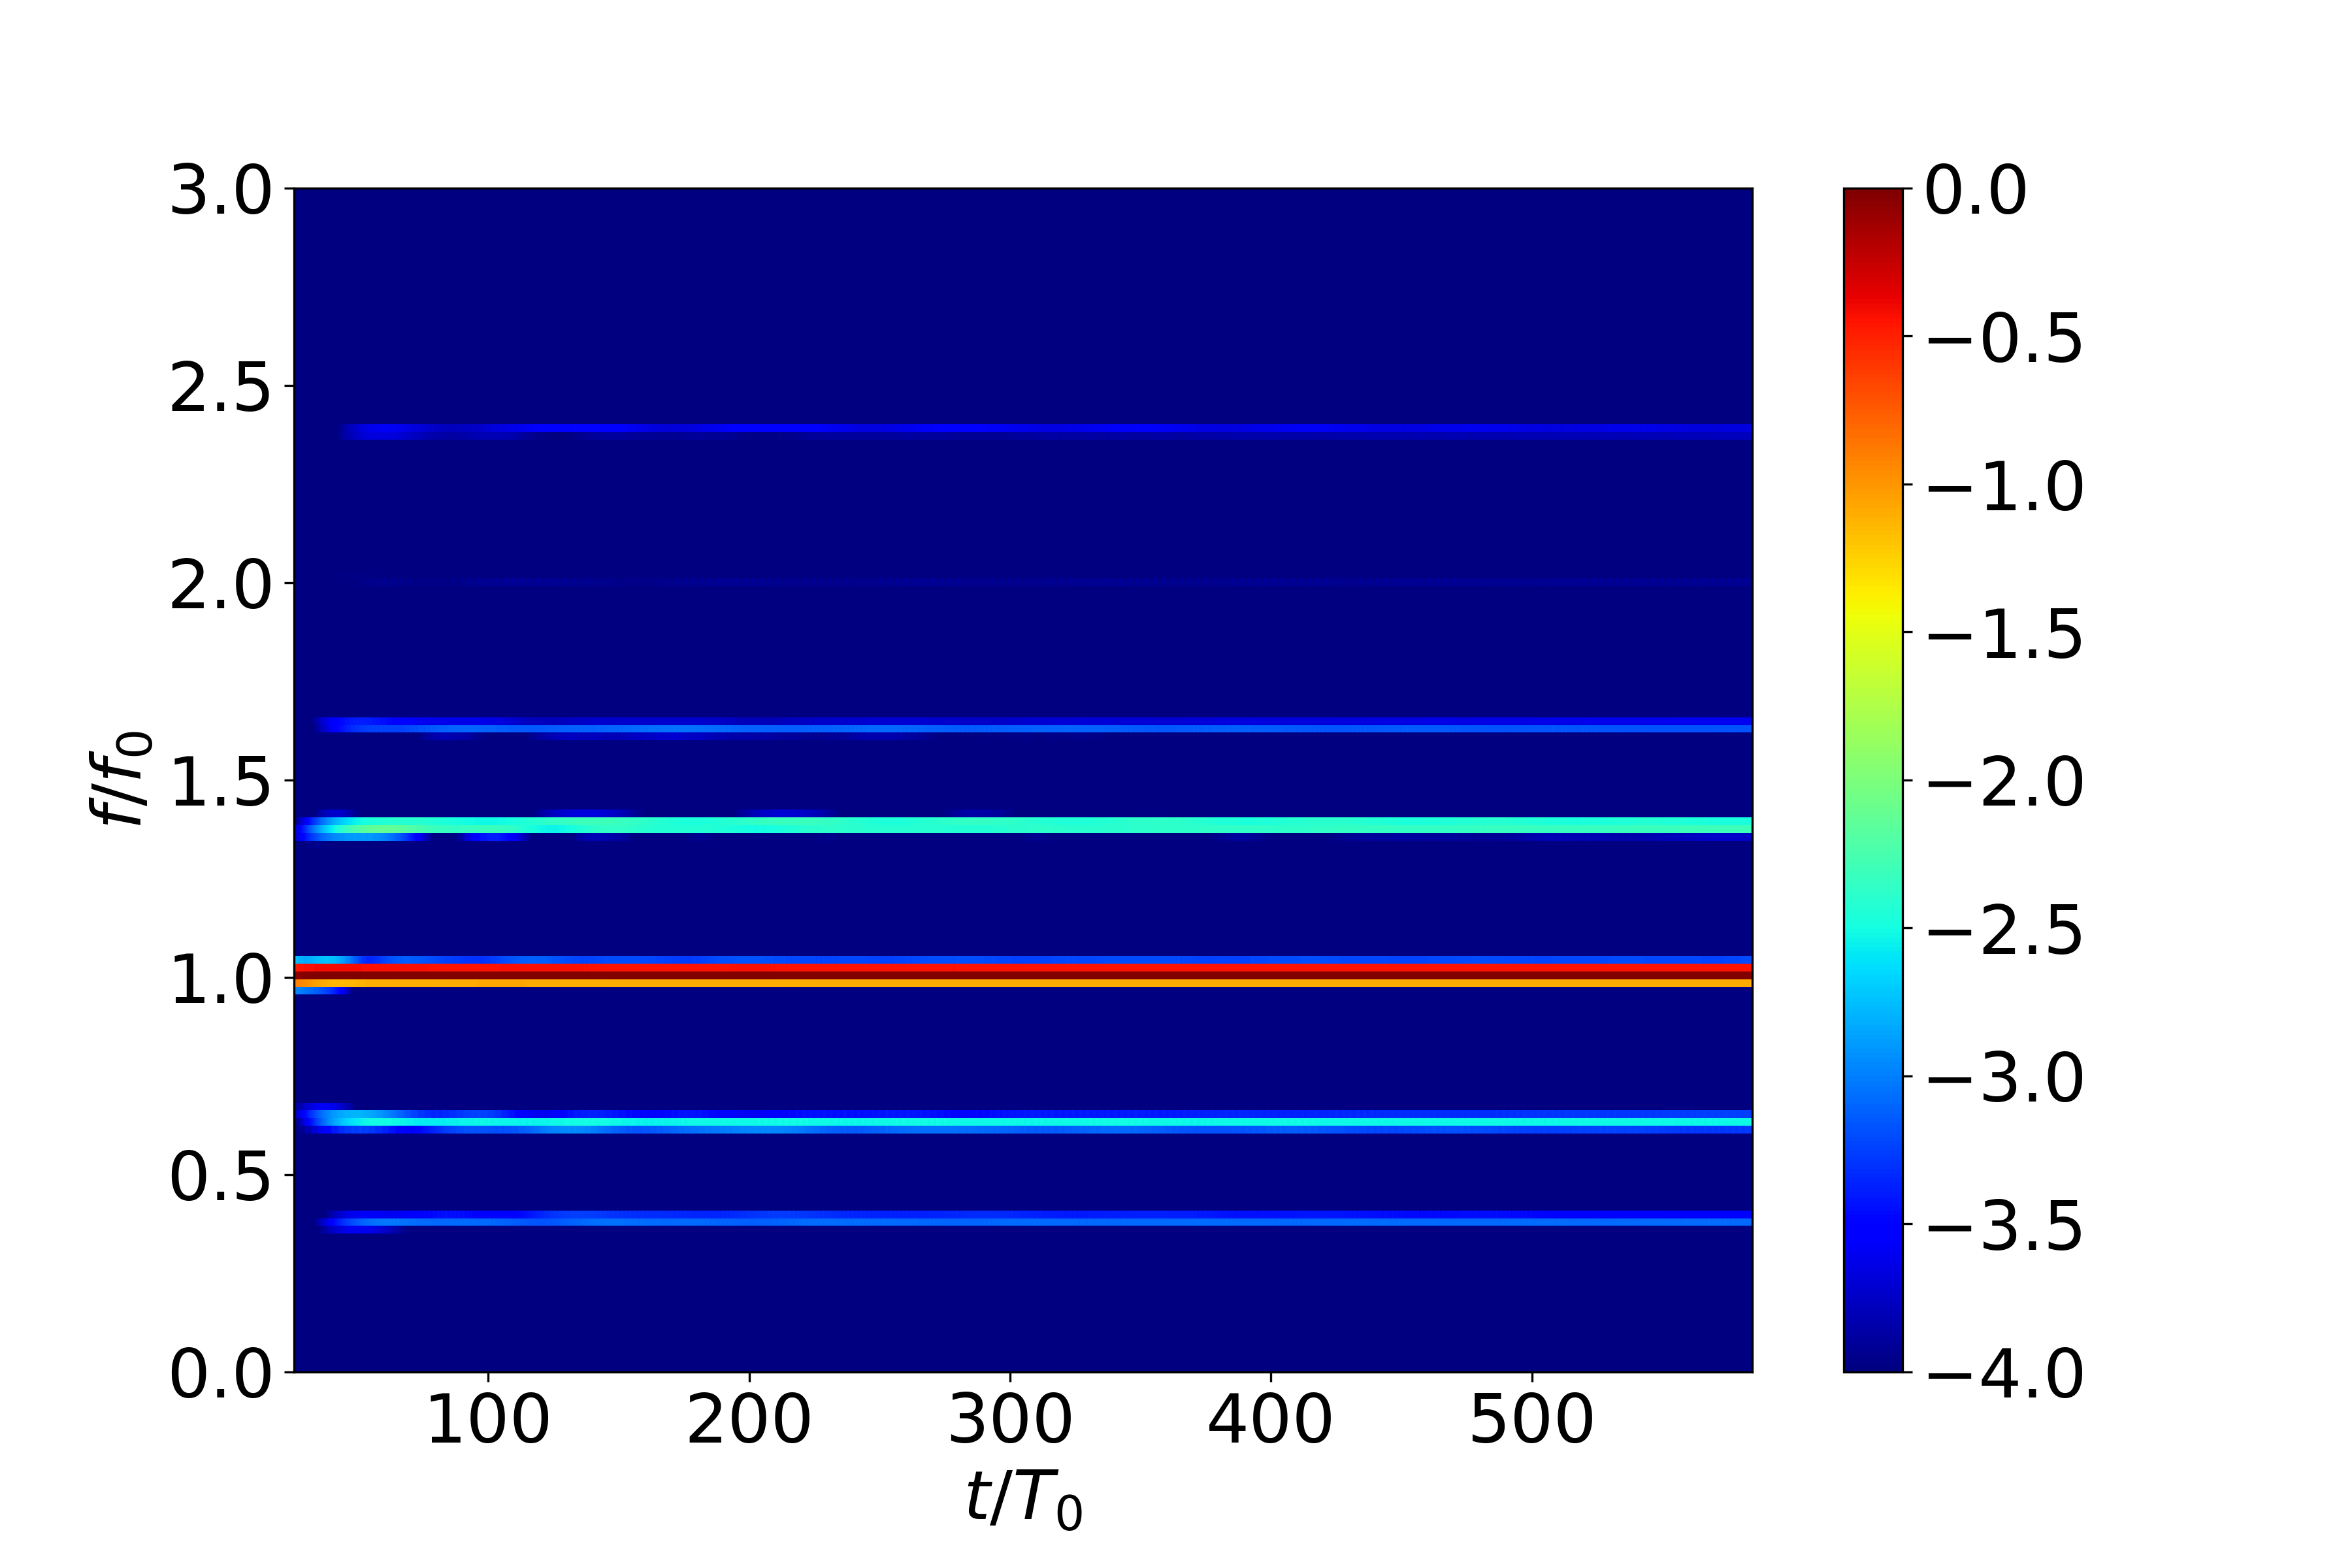
\includegraphics[width=1\textwidth]{{pics/H40L60N1ap05dp20w0p63/TFspectrumX35.6Y11.2N1024}.png}
	    \caption{Частотно-временная диаграмма}
	\end{subfigure}
	\caption{Характерная картина течения при монохроматическом воздействии }
	\label{fig:Vyamp05}
\end{figure}

\begin{table}
	\caption{ Кинетическая энергия при монохроматических воздействиях с амплитудой $a=0.02 cm$}. 
	\begin{center}
		\begin{tabular}{|c|c|c|c|c|c|}
			\hline
			$\displaystyle \frac{\omega_0}{N}$ & $E_k $ &  $<\overline{E}_{k}>$ & r\\
			0.55 ($\omega_{cr,1}$) & $1.32 \cdot 10^{-4}   $& 2.151    & 0.618     \\
			0.58                   & $8.45 \cdot 10^{-4}   $& 12.56    & 0.281     \\
			0.59                   & $ 12  \cdot 10^{-4}   $& 17.33    & 0.3       \\
			0.63                   & $29   \cdot 10^{-4}   $& 36.68    & 0.103     \\
			0.641                  & $23   \cdot 10^{-4}   $& 28.55    & 0.1129    \\
			0.66                   & $13.2 \cdot 10^{-4}   $& 15.14    & 0.152     \\
			0.70                   & $2.84 \cdot 10^{-4}   $& 2.896    & 0.295     \\
			0.74 ($\omega_{cr,2}$) & $1.50 \cdot 10^{-4}   $& 1.356    & 0.215     \\
			\hline
		\end{tabular}
	\end{center}
	\label{tab:bolts002}
\end{table}

При дальнейшем увеличении амплитуды возмущения до $a=0.1$см ($a/H=2.5\cdot 10^{-3}$) происходит развитие каскада триадных взаимодействий. Характерные картины волновых полей, спектров и развития во времени процесса колебаний и кинетической энергии системы приведены на рисунках \ref{fig:Vyamp1}. В частотном спектре сигнала доминируют дискретные компоненты, соответствующие частотам дочерних волн, возникающих при триадном резонансе аналогичные компонентам спектра, возникающим в слабонелинейном случае ($a/H=1.25\cdot 10^{-3}$). При этом полный спектр сигнала представляет собой суперпозицию дискретного и непрерывного спектра. Наличие непрерывного спектра свидетельствует о возникновении режима развитой волновой турбулентности \cite{Brouzet2016,Brouzetetal2017}. Соответствующие характеристики для кинетической энергии системы в сильно нелинейном режиме приведены в таблице \ref{tab:bolts01}. Из сопоставления таблиц \ref{tab:bolts002} и \ref{tab:bolts01} видно, что величины глобальных безразмерных энергетических характеристик системы (средней энергии  $<\overline{E}_{k}>$ и вариации относительно среднего $r$) в случае режима развитой волновой турбулентности слабо отличаются от безразмерных величин, характерных для линейного режима. Сопоставление волновых картин в линейном и нелинейном случаях показывает, что во втором случае энергия более равномерно распределена по изучаемой области: ветви аттрактора имеют большую ширину, а дочерние волны заполняют все пространство.

\begin{table}
	\caption{  Кинетическая энергия при монохроматических воздействиях с амплитудной $a=0.1 cm$. }
	\begin{center}
		\begin{tabular}{|c|c|c|c|c|}
			\hline
			$\displaystyle \frac{\omega_0}{N}$ & $E_k (erg)$ &  $<\overline{E}_{k}>$  & r\\
			%          $a$ &    $\displaystyle \frac{\omega_0}{N}$   & $E_k$ & ${E_k}/{\frac{(a\omega_0)^2}{2}}$ & $D_k$ & r\\
			0.55 ($\omega_{cr,1}$) & $33.0 \cdot 10^{-4}              $& 2.14  & 0.6193     \\
			0.63                   & $725 \cdot 10^{-4}              $& 36.7  & 0.1346     \\
			0.74 ($\omega_{cr,2}$) & $37.0 \cdot 10^{-4}              $& 1.35  & 0.2192     \\
			\hline
		\end{tabular}
	\end{center}
	\label{tab:bolts01}
\end{table}

Характерный пример волновой картины и основных качественных и количественных характеристик системы в линейном случае при бигармоническом внешнем воздействии приведен на рис.\ref{fig:biharmVyamp02} для следующих значений параметров: $\omega_1/N=0.58, \omega_2/N=0.66, a=0.02$см. Видно, что система выходит на режим квазистационарных биений за время порядка $40$ периодов колебаний, что близко к характерному времени выхода на процесс стационарных колебаний в монохроматическом случае. На частотном спектре доминируют пики, соответствующие частотам внешнего возмущения, имеются также пики, соответствующие частоте  $2\omega_1/N$ и разностной частоте $(\omega_2-\omega_1)/N$, но их величина более чем на два порядка меньше основного пика. Моменты времени, соответствующие максимальным значениям кинетической энергии, существенно отстают от моментов времени, соответствующих максимальным значениям амплитуды колебаний волнпродуктора. Важно отметить, что после выхода системы на режим установившихся биений средняя кинетическая энергия системы, возбуждаемой бигармоническим возмущением, с высокой точностью равна сумме энергий аттракторов, возбуждаемых монохроматическими возмущениями по отдельности $\overline{E}_{k}= { 21.7 \cdot 10^{-4}  }\approx \overline{E}_{k1}+\overline{E}_{k2}= (8.45+13.2) \cdot 10^{-4} = 21.65 \cdot 10^{-4}\, (erg/cm^2) $. Таким образом, в линейном режиме с высокой точностью соблюдается принцип линейной суперпозиции, что выполняется также при малой разности частот $(\omega_1-\omega_2)/N$. 

Примеры нелинейной динамики волновых аттракторов, генерируемых бигармоническими колебаниями волнопродуктора приведены на рис. \ref{fig:biharmVyap005-1} %\ref{fig:biharmVyap005-1-1} 
($\omega_1/N=0.66$, $\omega_2/N=0.628$, $\delta \omega/N=0.031$) и \ref{fig:biharmVyap005-2}, 
%\ref{fig:biharmVyap005-2-1} 
($\omega_1/N=0.628$, $\omega_2/N=0.641$, $\delta \omega/N=0.013$). Во всех случаях амплитуды колебаний волнопродуктора составили $a_{1}=a_{2}=0.05$см. Можно видеть, что в обоих случаях формируется движение, для которого характерен сложный частотный спектр, причем при уменьшении расстройки частот $\delta \omega$ наблюдается тенденция к более густому <<заселению>> спектра.  На графиках зависимости вертикальной скорости от времени виден характерный процесс <<биений>>. График зависимости кинетической энергии системы от времени показывает, что помимо колебаний среднего значения энергии имеет место нетривиальная динамика высокочастотных пульсаций энергии: на фазах роста и убывания огибающей амплитуды колебаний волнопродуктора амплитуды пульсаций могут отличаться на порядок. Таким образом, для нелинейного бигармонического режима характерны периодические <<вспышки>> волновой турбулентности. Такие <<вспышки>> хорошо видны на частотно-временных диаграммах, приведенных на рис.  \ref{fig:biharmVyap005-1} и \ref{fig:biharmVyap005-2}. В частности, на частотно-вереиенной диаграмме, приведенной на рис.  \ref{fig:biharmVyap005-1}, можно видеть, что <<биения>> амплитуды сигнала на частоте, близкой к частоте возмущающего воздействия, сдвинуты по времени относительно <<биений>> дочерних волн. Таким образом, <<биения>> огибающей колебаний волнопродуктора, <<биения>> средней кинетической энергии и <<вспышки>> волновой турбулентности рассогласованны между собой по времени. Можно предположить, что и в природных системах имеется рассогласование по времени между огибающей амплитуды внутреннего прилива и интенсификацией внутренней волновой турбулентности и перемешивания. Предварительное исследование энергии аттракторов, генерируемых бигармоническим возмущением, показывает, что в нелинейном случае средняя энергия системы существенным образом отличается от суммы энергий составляющих.  

\section*{Заключение к главе 3}

Для определения наиболее интересного диапазона параметров выполнено подробное исследование генерации аттракторов при монохроматическом возмущении, в результате чего определен частотный диапазон, в котором генерация аттракторов наиболее эффективна. Исследование поведения аттракторов при бигармоническом внешнем воздействии показало, что в линейном случае справедлив принцип суперпозиции: аттракторы, генерируемые каждой из компонент бигармонического возмущения практически не взаимодействуют друг с другом. В нелинейном случае при бигармоническом внешнем воздействии наблюдается режим биений, сопровождающийся вспышками волновой турбулентности, возникающей вследствие каскада триадных взаимодействий. При этом уровень пульсаций кинетической энергии на фазе роста огибающей амплитуды волнопродуктора, может на порядок превышать уровень, соответствующий спаду амплитуды колебаний волнопродуктора. 